% Szkielet dla pracy inżynierskiej pisanej w języku polskim.

\documentclass[polish,bachelor,a4paper,oneside]{ppfcmthesis}


\usepackage[utf8]{inputenc}
\usepackage[OT4]{fontenc}


% Authors of the thesis here. Separate them with \and
\author{%
Mateusz Bartos \album{122437} \and
Piotr Falkiewicz \album{122537} \and
Aleksandra Główczewska \album{122494} \and
Paweł Szudrowicz \album{122445}}
\title{System kontroli bezpieczeństwa – The Guard}                   % Note how we protect the final title phrase from breaking
\ppsupervisor{dr inż. Mariusz Nowak} % Your supervisor comes here.
\ppyear{2018}                                         % Year of final submission (not graduation!)


\begin{document}

    % Front matter starts here
    \frontmatter\pagestyle{empty}%
    \maketitle\cleardoublepage%

    % Blank info page for "karta dyplomowa"
    \thispagestyle{empty}\vspace*{\fill}%
    \begin{center}
        Tutaj przychodzi karta pracy dyplomowej;\\oryginał wstawiamy do wersji dla archiwum PP, w pozostałych kopiach wstawiamy ksero.
    \end{center}%
    \vfill\cleardoublepage%

    % Table of contents.
    \pagenumbering{Roman}\pagestyle{ppfcmthesis}%
    \tableofcontents* \cleardoublepage%

    % Main content of your thesis starts here.
    \mainmatter%
    \chapter{Wstęp}
Inspiracją niniejszego projektu była chęć ulepszenia istniejących systemów monitoringu o nowoczesne mechanizmy powszechnie używane w projektach programistycznych.
Nowoczesne systemy kontroli bezpieczeństwa powinny nie tylko nagrywać obraz ale także analizować go w czasie rzeczywistym i odpowiednio reagować. Na podstawie danych z kamer i czujników system powinien podejmować decyzje o stanie bezpieczeństwa domu i alarmować użytkownika o wykrytych zagrożeniach.

System kontroli bezpieczeństwa - The Guard jest naszą odpowiedzią na przedstawione problemy. Naszym celem było stworzenie systemu umożliwiającego analizę danych z czujników pomiarowych, monitorowanie pomieszczeń, w których zamontowano nasz system a także nagrywanie materiału video w momencie wykrycia ruchu i przechowywaniu go bezpiecznie na zewnętrznym serwerze aby był dostępny dla nas w każdym momencie i nie uległ zniszczeniu. Zadaniem systemu jest także poinformowanie o każdym niebezpieczeństwie właściciela systemu. Priorytetem był prosty i intuicyjny program obsługi, który mógłby być użyty przez każdą osobę, na każdej z najbardziej popularnych platform. Zdecydowano się na aplikację internetową i dwie aplikacje mobilne napisane natywnie dla systemu iOS i Android. Ponadto uzgodniono, że rozwiązanie będzie oparte na niezależnych modułach, które będzie można później, w łatwy sposób, zmodyfikować. Całość pracy jest na licencji open-source, aby każdy użytkownik mógł nie tylko korzystać z systemu ale także dowolnie go edytować.

W ramach pracy przygotowano projekt całego systemu, od urządzeń zbierających dane, przez system monitorujący i analizujący zebrane dane, po aplikacje klienckie. Następnie zaimplementowano zaprojektowane wcześniej aplikacje, złożono zestawy urządzeń składających się z Raspberry Pi 3 i czujników, oraz połączono wszystkie elementy w jeden spójny system.
Ze względu na cel pracy oraz wykorzystane technologie i usługi, zespół oparł swoją pracę o: dokumentację usług dostępną na stronach internetowych producentów, dokumentację narzędzi dołączoną do odpowiednich repozytoriów, dokumentację sprzętu.

\paragraph{Podział pracy}
\begin{itemize}
\item Mateusz Bartos: \\
Zaprojektował architekturę systemu, stworzył aplikację mobilną przeznaczoną na system Android. Ponadto przygotował maszynę wirtualną w ramach usług oferowanych przez chmurę Microsoft Azure.
\item Piotr Falkiewicz: \\
Wykonał projekt serwera obsługującego aplikacje mobilne w oparciu o protokół HTTP oraz był odpowiedzialny za przetwarzanie monitoringu dostarczanego w czasie rzeczywistym z urządzeń do aplikacji przy wykorzystaniu modułu Nginx RTMP.
\item Aleksandra Główczewska: \\
Zaprojektowała i wykonała aplikację internetową z wykorzystaniem języka Python i biblioteki Django. Odpowiedzialna za wprowadzenie uwierzytelniania użytkowników.
\item Paweł Szudrowicz: \\
Przygotował urządzenia oparte na Raspberry Pi 3 do obsługi czujników i wykonał oprogramowanie pracujące na każdym z nich. Zaprojektował i wykonał aplikację mobilną przeznaczoną na urządzenia iOS a także zaimplementował obsługę push notyfikacji wykorzystując do tego usługi Firebase.
\end{itemize}

\paragraph{Struktura pracy}
W pierwszym rozdziale opisano architekturę przygotowanego systemu. Następna część poświęcona jest opisowi kosztów utrzymania działającego systemu i wszystkich wymaganych podzespołów do jego poprawnej pracy. Kolejny dział zawiera specyfikację wykorzystanych czujników i schemat poprawnego ich podłączenia a także informacje dot. przetwarzania obrazu. W części tej poruszono również kwestię poprawnej instalacji oprogramowania na urządzeniu Raspberry Pi 3.  W czwartej części zaprezentowano użyte rozwiązania chmurowe takie jak Microsoft Azure, Firebase i omówiono działanie naszego serwera opartego na Django. Aplikacje klienckie są kolejnym tematem tej pracy. Do ich opisania wykorzystano zdjęcia ekranów z działających aplikacji i wytłumaczono najważniejsze aspekty w ich realizacji. W ostatnim dziale opisano przeprowadzone testy funkcjonalne.

    \chapter{Architektura systemu}

Wstęp do rozdziału

\section{Schemat}

// Piotr - schemat na podstawie "Praca inżynierska na Google Docs"
//tzn?

\section{Komunikacja}

Komunikacja, pomiędzy elementami systemu, odbywa się na zasadach architektury REST. Takie podejście gwarantuje prostotę przesyłanych komunikatów oraz skalowalność w kontekście nowych urządzeń Raspberry, strumieniujących dane, oraz nowych urządzeń korzystających z aplikacji klienckich. Początkowo, projekt był oparty o zapytania GET i POST.  

\paragraph{Zapytanie GET}
Metoda GET pozwala na pobranie dokumentu sieciowego, na postawie zapytania zawartego w adresie URL. Metoda ta jest używana tylko i wyłącznie do pobierania danych z punktu docelowego. 

\paragraph{Zapytanie POST}
W metodzie POST, należy zamieścić wiadomość wewnątrz zapytania HTTP. Odpowiedzią na ten typ zapytania, może być zarówno kod statusu, jak i dane, zwracane w podobnej postaci jak przy zapytaniu GET.

Wprowadzenie tokenów uwierzytelniających (więcej w akapicie nt. Bezpieczeństwa), spowodowało, że wymianę komunikatów oparto tylko i wyłącznie na zapytaniach POST. 
W zależności od zadania, obsługa zapytania polega na wykonaniu zapytania na bazie danych lub wysłaniu notyfikacji do klienta.
Obsługę zapytań można również podzielić, ze względu na zaplanowane źródło zapytania: aplikacja użytkownika lub urządzenie Raspberry.
W pierwszej kolejności przedstawione zostaną wiadomości wymieniane na linii Raspberry - Serwer.
\paragraph{a) Rejestracja Raspberry Pi:}
\begin{verbatim}
Adres: /backend/v1/devices/add
Zawartość:
{
	'serial': <serial-urządzenia>, 
	'name': <nazwa-urządzenia>, 
	'token': 'jwt.token.from.client'
}
\end{verbatim}
Działanie: Raspberry, o podanych serialu i nazwie, zostaje dodane do bazy danych urządzeń.

\paragraph{b) Wykrycie ruchu:}
\begin{verbatim}
Adres: /backend/v1/PIRnotification
Zawartość: 
{
	'serial': <serial-urządzenia>, 
	'message': <wiadomość>, 
	'token': 'jwt.token.from.client'
}
\end{verbatim}
Działanie: Po odebraniu informacji, o wykryciu ruchu, następuje pobranie klatki ze strumienia obrazu, nadawanego przez Raspberry o wskazanym serialu. Jeśli wykryto ruch człowieka, następuje nagranie fragmentu wideo, który zostaje zapisany w bazie danych Firebase Storage, a użytkownik zostaje poinformowany o zajściu i o nagraniu, któe może pobrać. Jeśli nie wykryto obecności ludzkiej, notyfikacja zostaje zignorowana.

\paragraph{c) Wykrycie zmian na czujniku:}
\begin{verbatim}
Adres: /backend/v1/notification
Zawartość: 
{
	'serial': <serial-urządzenia>, 
	'sensorType': <typ-czujnika>, 
	'value': <wartość>, 
	'token': `jwt.token.from.client`
}
\end{verbatim}
Działanie: Informuje serwer o zmianie wartości jednego z czujników.\newline
Następne zapytania dotyczą poleceń wysyłanych z aplikacji użytkownika.
\paragraph{d) Pobranie urządzeń użytkownika:}
\begin{verbatim}
Adres: /backend/v1/get
Zawartość: 
{
	'owner':<użytkownik>, 
	'token': 'jwt.token.from.client'
}
\end{verbatim}
Działanie: Zwraca listę urządzeń użytkownika.
\paragraph{e) Zmiana nazwy urządzenia:}
\begin{verbatim}
Adres: /backend/v1/devices/changeRaspName
Zawartość:
{
	'serial': <serial-urządzenia>, 
	'name': <nowa-nazwa>, 
	'token': 'jwt.token.from.client'
}
\end{verbatim}
Działanie: Zmienia nazwę urządzenia, wyświetlaną w podglądzie, w aplikacji użytkownika.
\paragraph{f) Uzbrojenie/rozbrojenie urządzenia:}
\begin{verbatim}
Adres: /backend/v1/devices/changeIsArmed
Zawartość: 
{
	'serial': <serial-urządzenia>, 
	'armed': <nowy-stan>, 
	'token': 'jwt.token.from.client'
}
\end{verbatim}
Działanie: Ustala, czy nowe powiadomienia, związane z urządzeniem, dalej będą wysyłane do aplikacji.
\paragraph{g) Pobranie listy notyfikacji:}
\begin{verbatim}
Adres: /backend/v1/devices/getNotifications
Zawartość: 
{
	'serial': <serial-urządzenia>,  
	'token': 'jwt.token.from.client'
}
\end{verbatim}
Działanie: Pobiera listę notyfikacji, powiązanych z urządzeniem o podanym serialu.
\paragraph{h) Powiązanie aplikacji z kontem użytkownika:}
\begin{verbatim}
Adres: /backend/v1/devices/fcmTokenUpdate
Zawartość: 
{
	'email': <użytkownik>, 
	'fcmToken': <token-z-firebase>, 
	'deviceId' : <id_aplikacji>
}
\end{verbatim}
Działanie: Powiązuje aplikację, zarówno mobilną, jak i sesję aplikacji przeglądarkowej, o podanym tokenie, z kontem użytkownika. Dzięki temu, notyfikacje trafiają na wszystkie urządzenia użytkownika.
\newline
\newline
Wybrane rozwiązanie pozwala na łatwą lokalizację ewentualnego błędu w działaniu systemu, oraz szybką naprawę zaistniałego problemu. Ponadto prosta logika oraz łatwe, krótkie funkcje, obsługujące zapytania, sprawiają, że dalszy rozwój tej części systemu, będzie możliwy bardzo niskim nakładem sił. 

\section{Bezpieczeństwo}

Aplikacje wysyłając zapytania do serwera, muszą potwierdzić swoją tożsamość, co dzieje się inaczej w przypadku aplikacji mobilnych i aplikacji webowej.

W~przypadku aplikacji mobilnych zastosowano proponowane przez Firebase rozwiązanie JSON Web Tokens. W~momencie wysłania zapytania POST do serwera, aplikacja wysyła także unikalny token, który następnie jest przez serwer weryfikowany przy użyciu Firebase Admin SDK.

W~przypadku aplikacji internetowej, zastosowano wbudowane w bibliotekę Django zabezpieczenia: CSRF token oraz przesyłanie id sesji wraz z zapytaniem. Zabezpieczenie CSRF tokenem uniemożliwia tzw. `Cross Site Request Forgery' tj. ataki w~których na stronie, gdzie zalogowany jest użytkownik bez jego wiedzy uruchamiany jest skrypt, najczęściej w języku JavaScript. Następnie, korzystając z~faktu, że użytkownik jest zalogowany, wysyłane jest zapytanie na serwer, które może zrobić wszystkie operacje do których upoważniony jest dany użytkownik. CSRF token zapisywany jest w przeglądarce jako `ciasteczko' (eng. cookie) i jest dołączany do danych przesyłanych w momenie kliknięcia przycisku odpowiedzialnego za przesłanie formularza. Następnie wbudowana w serwer Django biblioteka weryfikuje na podstawie zapisanych i przesłanych danych sesji poprawność tokenu i w przypadku błędu zwraca błąd serwera 403.
Ponieważ token przy każdym zapytaniu jest tworzony na nowo na podstawie otwartej sesji, rozwiązanie nie było komfortowe dla użytkowników aplikacji mobilnych: aplikacja musiałaby najpierw ustanowić połączenie z serwerem (wysłać zapytanie GET na stronę główną), następnie zalogować się (wysłać zapytanie POST z danymi logowania) oraz zapisywać tokeny i id sesji odsyłane przez serwer. Aby ograniczyć ilość zapytań wysyłanych do serwera, posłużono się powyżej opisaną metodą tokenów JWT.

    \chapter{Zbieranie i przetwarzanie danych z czujników}
\section*{Raspberry Pi}
<<<<<<< HEAD

Wszystkie zestawy zbudowano w oparciu o Raspberry Pi 3 v1.2 (rys. 3.1). Zdecydowano się na to rozwiązanie, ponieważ bazuje on na dystrybucji Linuxa, posiada opowiednie interfejsy i złącza a także zintegrowany moduł WiFi. Minusem w stosunku do konkurencyjnego Arduino jest brak wejść analogowych. Problem rozwiązano dodając zewnętrzny przetwornik A/C.
=======
Wszystkie zestawy zbudowano w oparciu o Raspberry Pi 3 v1.2. Zdecydowano się na to rozwiązanie, ponieważ bazuje on na dystrybucji Linuxa, posiada opowiednie interfejsy i złącza a także zintegrowany moduł WiFi. Minusem w stosunku do konkurencyjnego Arduino jest brak wejść analogowych. Problem rozwiązano dodając zewnętrzny przetwornik A/C. Całość zamknięto w małą plastikową obudowę z wyciętymi otworami na czujniki (rys. 3.1). Schemat budowy układu wykonano w programie Fritzing (rys. 3.2).
\begin{figure}[h]
	\centering
	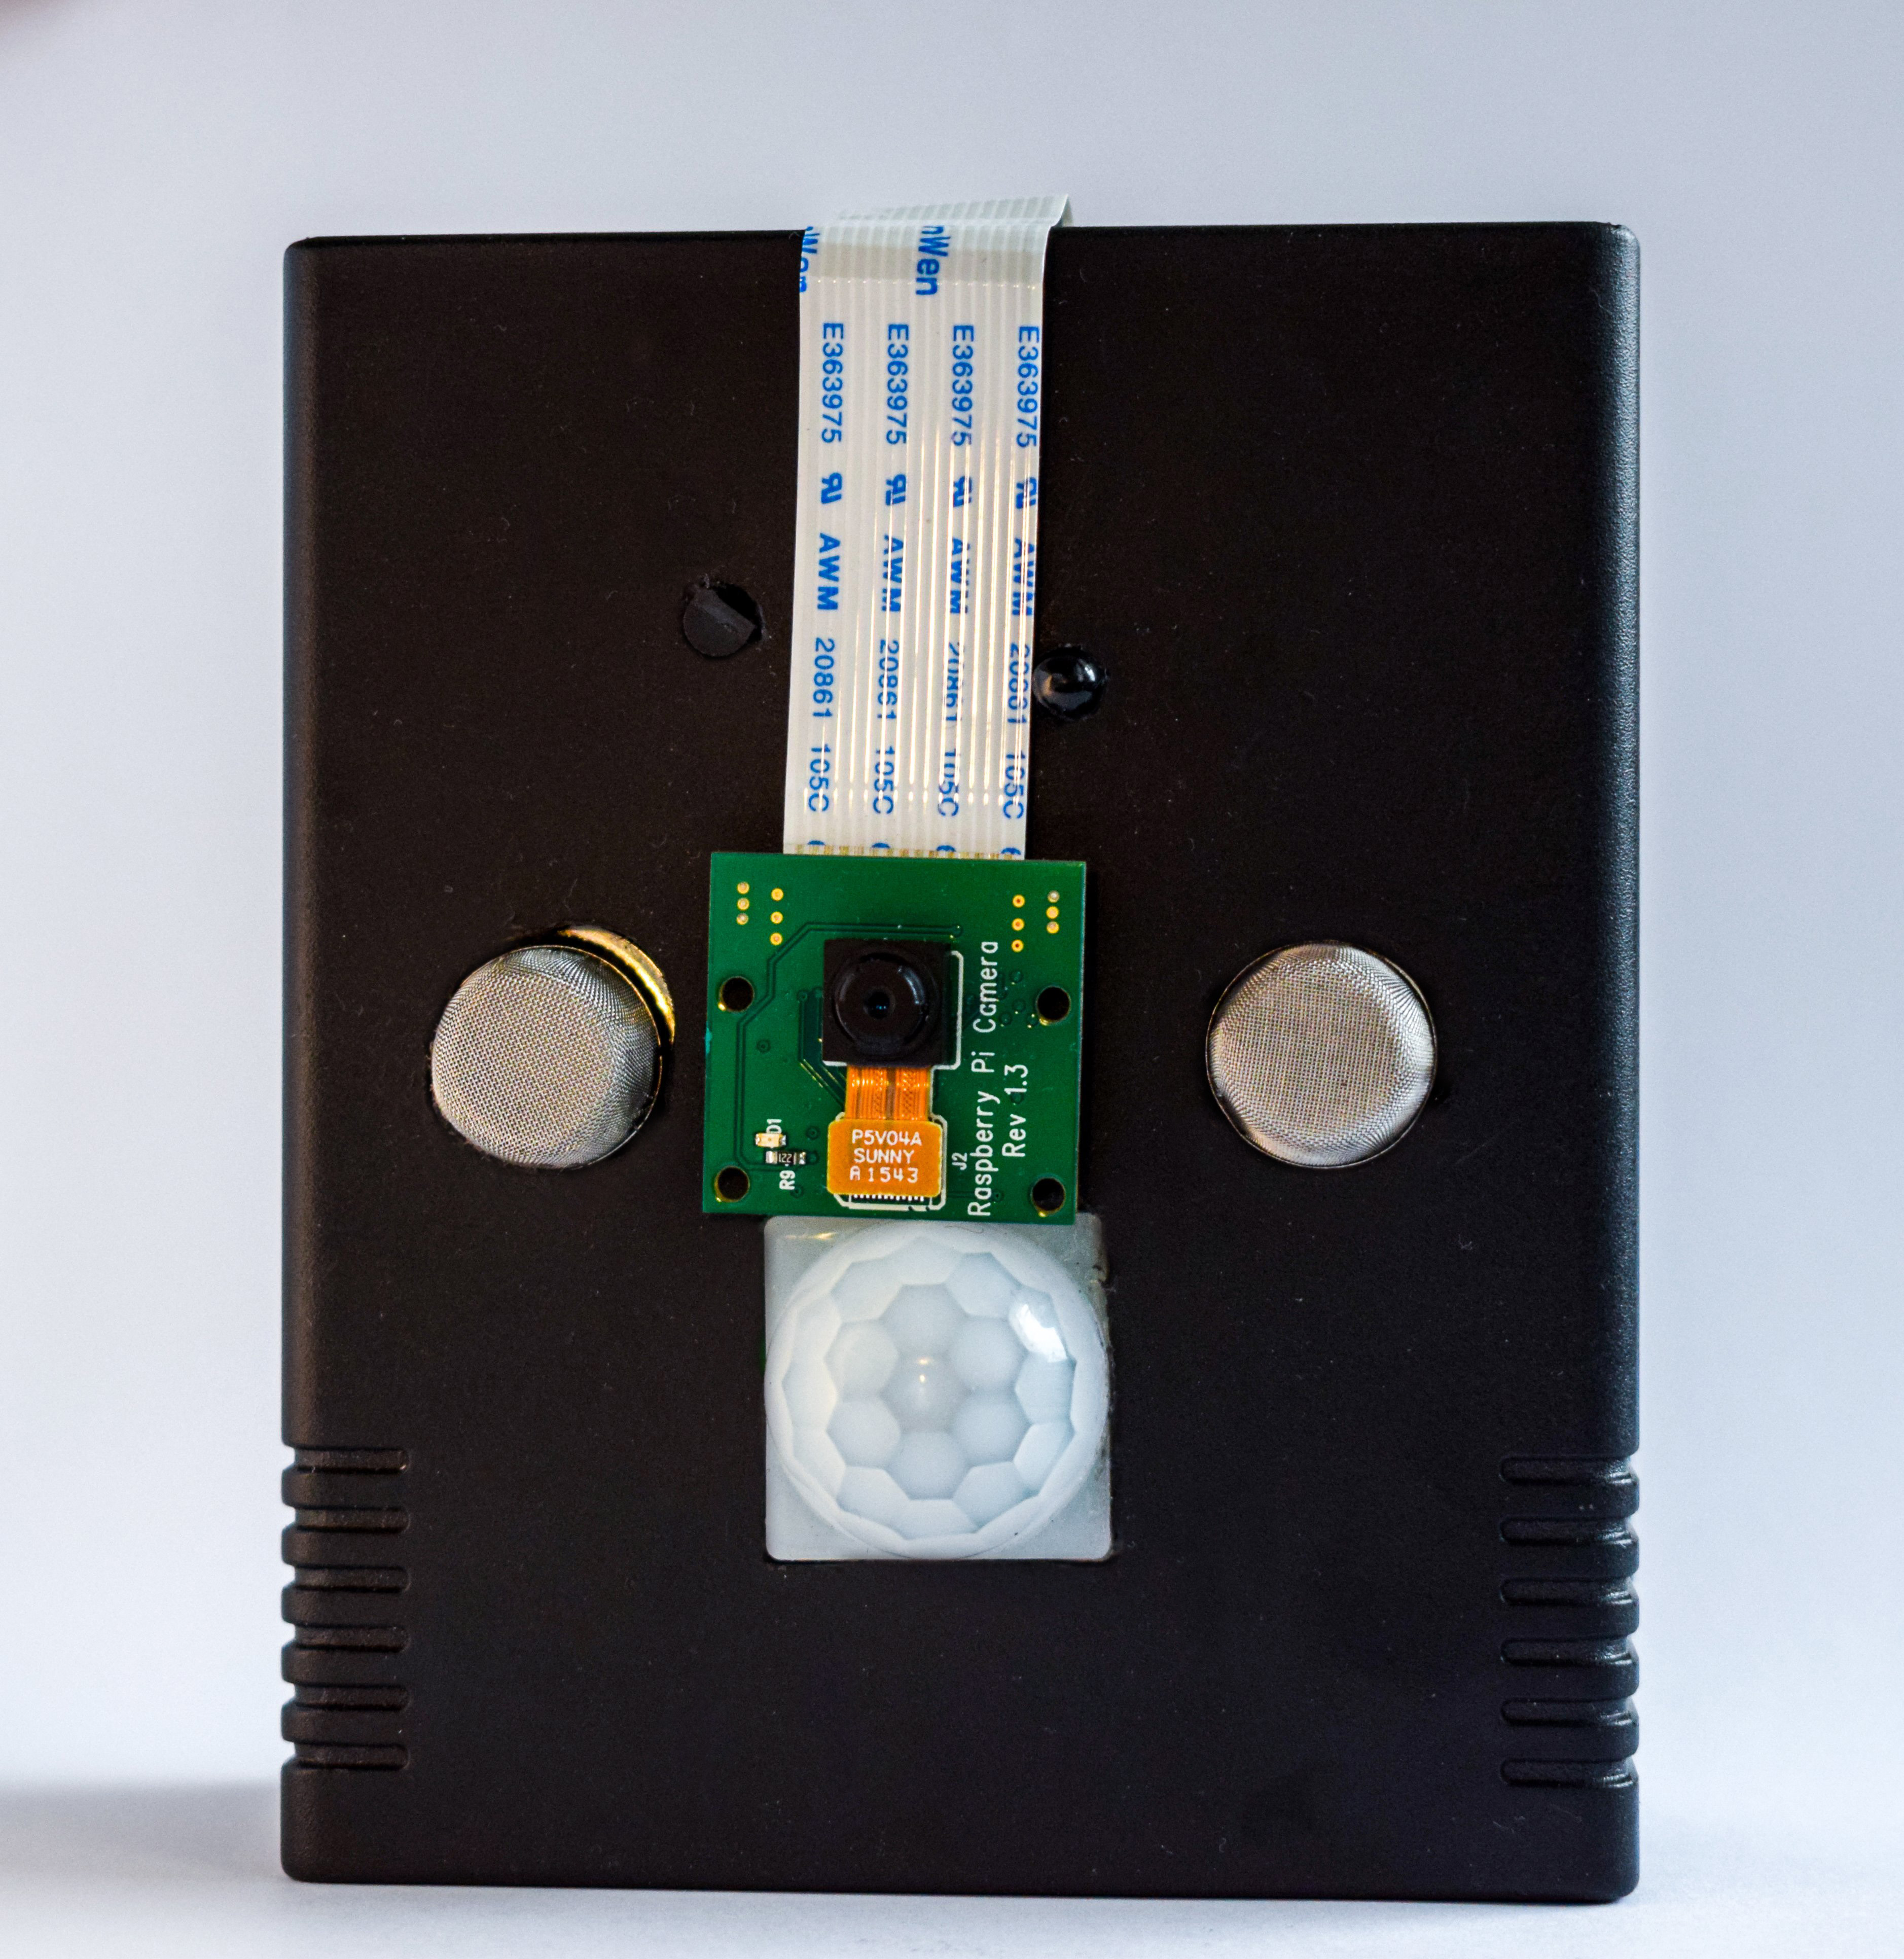
\includegraphics[width=7cm]{guard.jpg}
	\caption{Zbudowany zestaw The Guard}
\end{figure}
\begin{figure}[h]
	\centering
	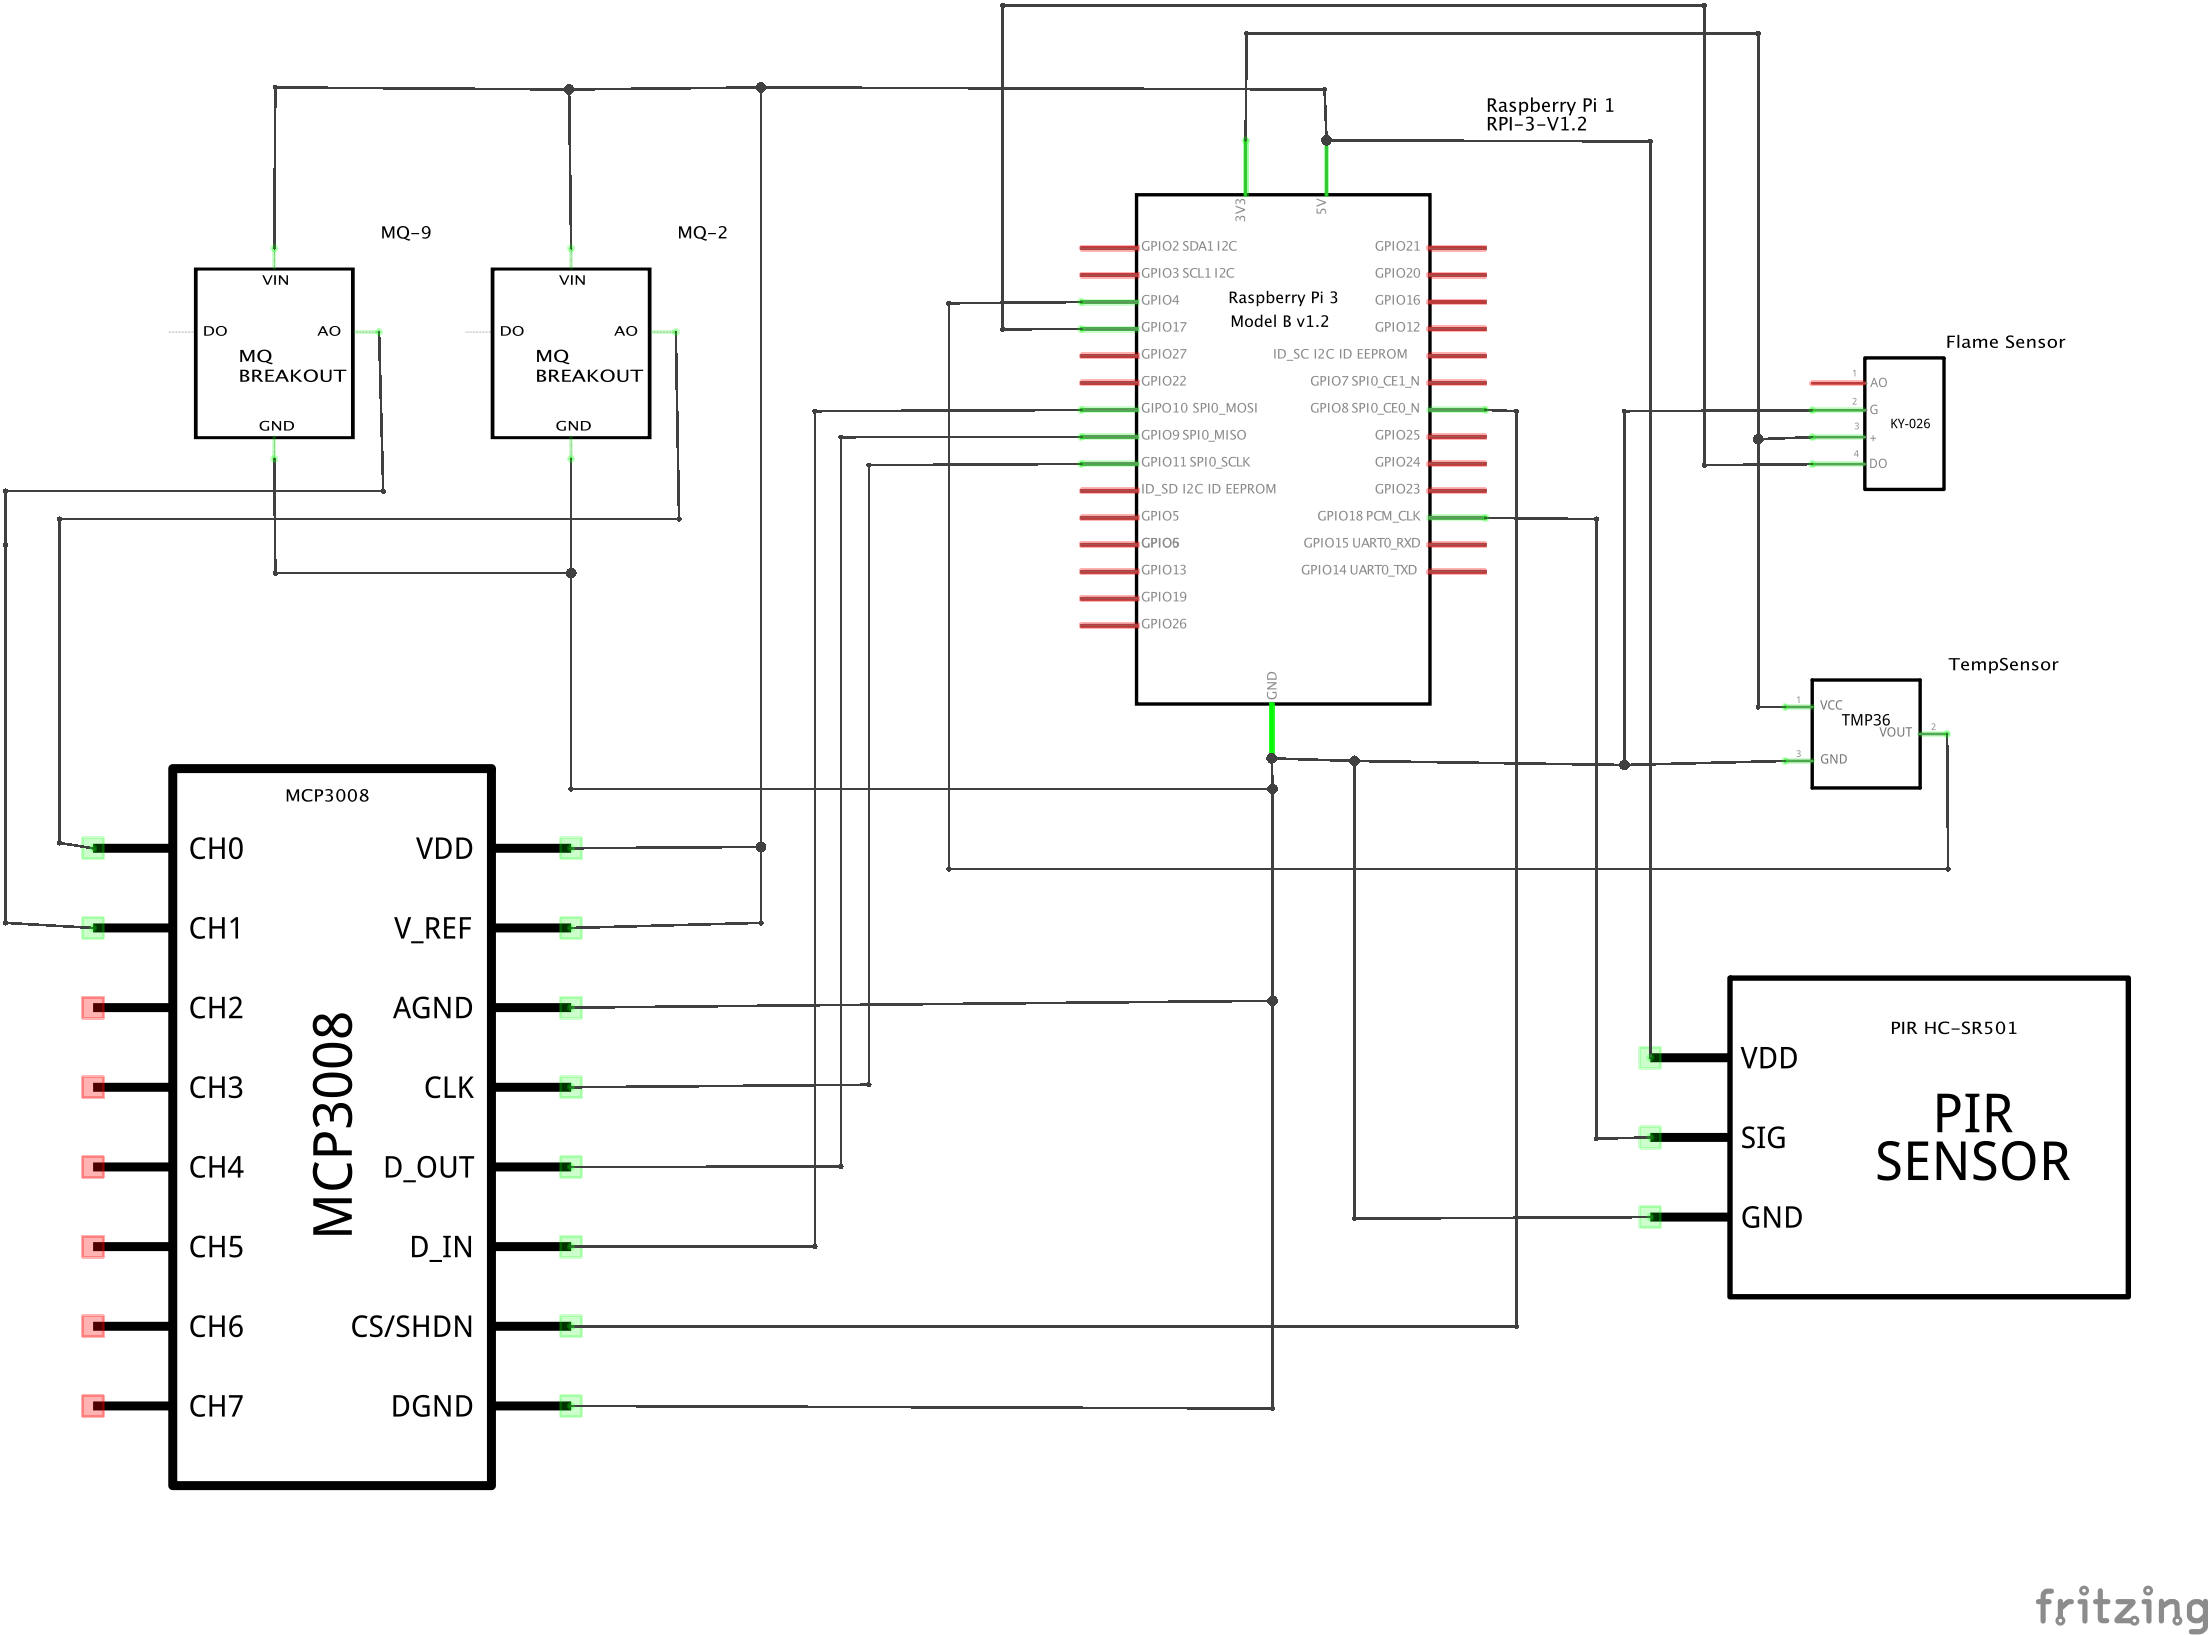
\includegraphics[width=15cm]{GuardSchem}
	\caption{Schemat układu The Guard}
\end{figure}
>>>>>>> 2688ba13846a92baa8deea770d60be5065fe7915
\paragraph{Specyfikacja Raspberry Pi 3:}
\begin{itemize} 
\item Procesor 1.2 GHz
\item Liczba rdzeni 4. Quad Core
\item Pamięć RAM 1 GB
\item Pamięć Karta microSD
\item 40 GPIO
\end{itemize}
Aby prawidłowo zainstalować oprogramowanie The Guard na dowolnym urządzeniu Raspberry Pi 3 należy wykonać poniższe czynności w terminalu:
\begin{enumerate} 
\item sudo apt-get install libx264-dev
\item cd /usr/src
\item git clone git://source.ffmpeg.org/ffmpeg.git
\item sudo ./configure --arch=armel --target-os=linux --enable-gpl --enable-libx264 --enable-nonfree
\item sudo make
\item sudo install
\item sudo nano /boot/config.txt
\item w pliku config.txt dopisać Dtoverlay=w1-gpio i Gpiopin=4
\item pip intall wiringpi
\item sudo pip install spidev
\item pip install pyrebase
\end{enumerate}
<<<<<<< HEAD
Następnym krokiem jest włączenie odpowiednich interfejsów w panelu konfiguracyjnym. Należy zmienić ustawienia zgodnie ze schematem 3.2:
\begin{figure}[h]
=======
Następnym krokiem jest włączenie odpowiednich interfejsów w panelu konfiguracyjnym. Należy zmienić ustawienia zgodnie ze schematem (rys. 3.3).
\begin{figure}[ht]
>>>>>>> 2688ba13846a92baa8deea770d60be5065fe7915
	\centering
	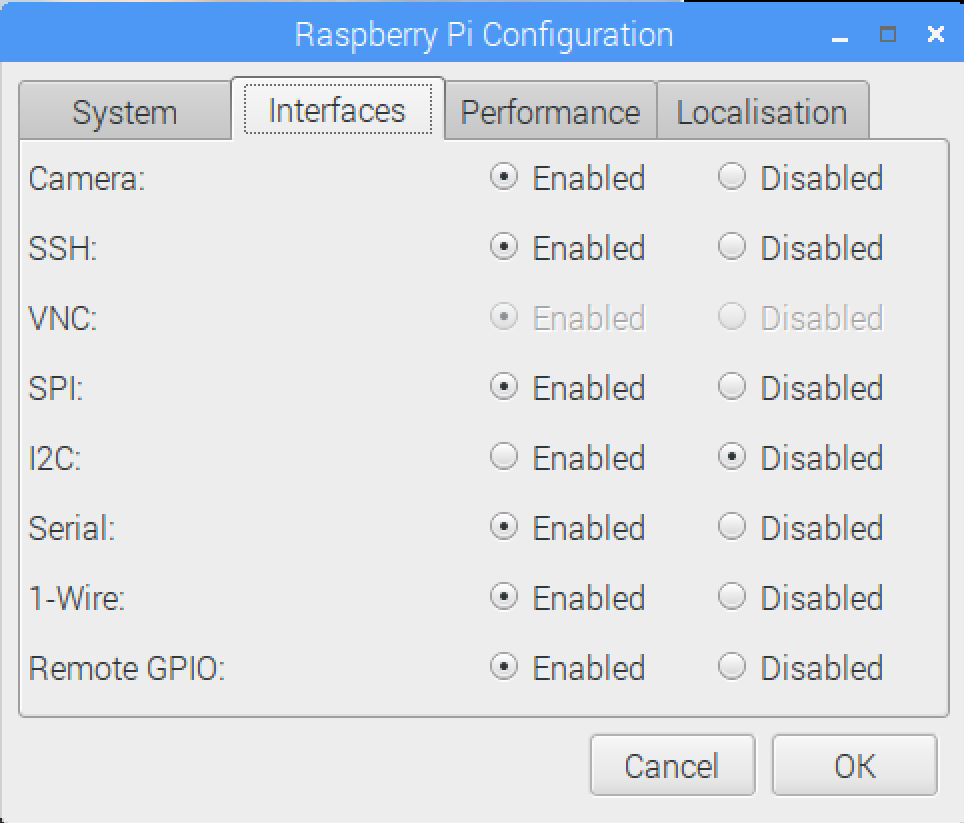
\includegraphics[width=6cm]{RSettings}
	\caption{Ustawienia}
\end{figure}
<<<<<<< HEAD
W kodzie użyto biblioteki wiringpi do odczytu danych z układów cyfrowych. Należy podkreślić, że numeracja fizycznych pinów(rys. 3.4) i numeracja pinów w bibliotece wiringPi(rys. 3.3) jest różna i nie zawiera wszystkich dostępnych pinów na urządzeniu. Przykładowo odczyt pinu numer 1 w wiringPi jest równoznaczny z odczytem stanu na pinie numer 12 (GPIO18).
\begin{figure}[h]
=======
Użyto biblioteki wiringpi do odczytu danych z układów cyfrowych. Należy podkreślić, że numeracja fizycznych pinów(rys. 3.4) i numeracja pinów w wiringPi(rys. 3.5) jest różna i nie zawiera wszystkich dostępnych pinów na urządzeniu. Przykładowo odczyt pinu numer 1 w wiringPi jest równoznaczny z odczytem stanu na pinie numer 12 (GPIO18).
\begin{figure}[ht]
>>>>>>> 2688ba13846a92baa8deea770d60be5065fe7915
  \centering
  \begin{minipage}[b]{0.4\textwidth}
    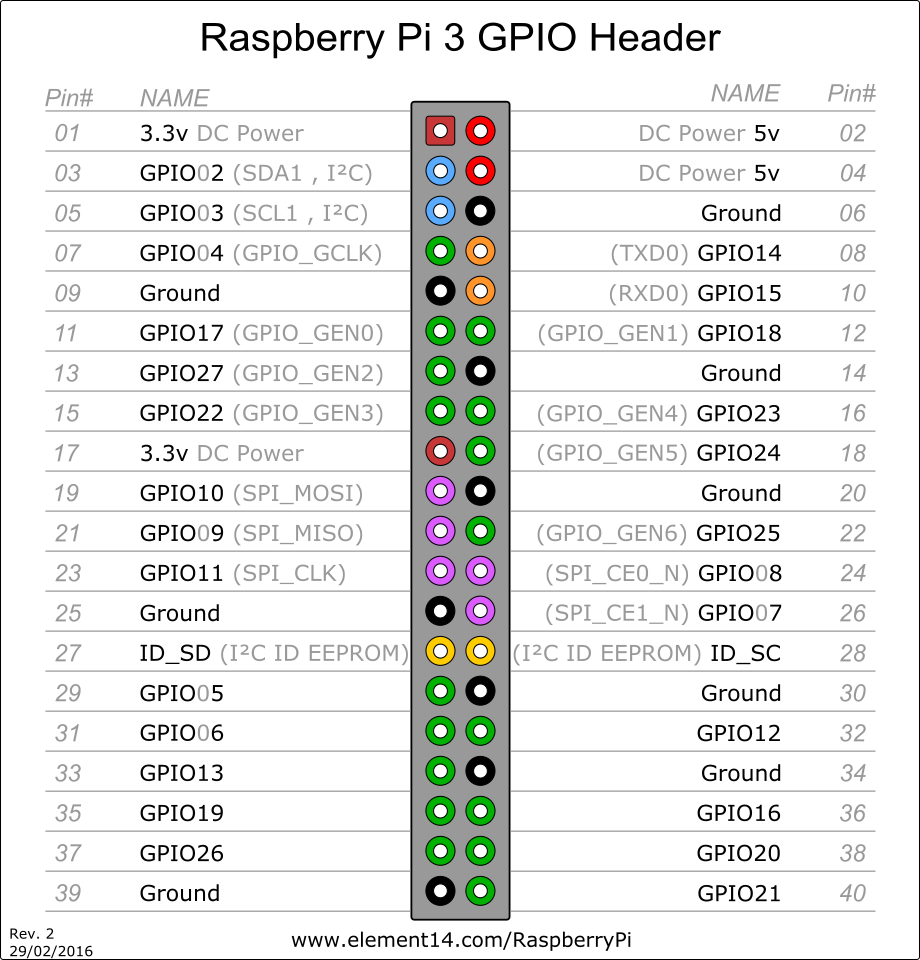
\includegraphics[width=\textwidth]{gpio.png}
    \caption{GPIO}
  \end{minipage}
  \hfill
  \begin{minipage}[b]{0.4\textwidth}
    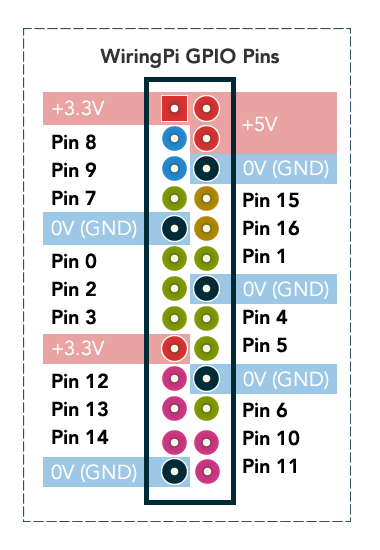
\includegraphics[width=\textwidth]{wiringpi.png}
    \caption{WiringPi}
  \end{minipage}
\end{figure}
Zainstalowane oprogramowanie odpowiedzialne jest za ciągłe monitorowanie stanów i zbieranie danych z czujników pomiarowych. Po podłączeniu układu do zasilania program jest uruchamiany automatycznie. Pierwszą czynnością jaką wykonuje Raspberry Pi jest wysłanie swojego numeru seryjnego do bazy danych Firebase. Cały proces jest w pełni zautomatyzowany. Dzięki temu użytkownicy od razu mogą dodać urządzenie i przeglądać dane z czujników na aplikacjach klienckich. Dodanie akcesorium pomiarowego następuje poprzez wprowadzenie w aplikacji jego numeru seryjnego.
\section*{Czujniki}
Każdy zestaw składa się z 5 czujników analogowo cyfrowych,  jednej kamery i jednego przetwornika AC. 
\paragraph{a) Specyfikacja MQ-9 - czujnik tlenku węgla:}
\begin{itemize} 
\item Zasilanie: 5 V
\item Pobór prądu: 150 mA
\item Temperatura pracy: od -10 do 50 \textdegree{}C
\item Wyjścia: analogowe oraz cyfrowe
\end{itemize}
\paragraph{b) Specyfikacja MQ-2 - czujnik LPG i dymu:}
\begin{itemize} 
\item Zasilanie: 5 V
\item Pobór prądu: 150 mA
\item Temperatura pracy: od -10 do 50 \textdegree{}C
\item Wyjścia: analogowe oraz cyfrowe
\end{itemize}
\paragraph{c) Specyfikacja czujnika wykrywania płomieni:}
\begin{itemize} 
\item Zasilanie: 3.3 V
\item Zakres wykrywanej fali: 760 do 1100nm
\item Kąt detekcji: od 0 do 60 stopni
\item Temperatura pracy: od -25 do 85 \textdegree{}C
\end{itemize}
\paragraph{d) Specyfikacja DS18B20 - czujnik temperatury:}
\begin{itemize} 
\item Zasilanie: 3.3 V
\item Zakres pomiarowy: od -55 do 125 \textdegree{}C
\end{itemize}
\paragraph{e) Kamera:}
\begin{itemize} 
\item Wykorzystano moduł kamery Raspberry Pi element14
\item Kamera 5MP - wspierająca nagrywanie 30 klatek na sekundę w rozdzielczości Full HD
\end{itemize}
\paragraph{f) Specyfikacja MCP3008 - przetwornik A/C:}
\begin{itemize} 
\item Zasilanie: od 2.7V do 5.5V
\item Pobór prądu: 0.5 mA
\item Interfejs komunikacyjny: SPI
\item Liczba kanałów: 8
\item Rozdzielczość: 10bit
\item Czas konwersji: 10us
\end{itemize}
<<<<<<< HEAD
\begin{figure}[h]
=======
Na schematach (rys. 3.6, rys. 3.7) przedstawiono charakterystykę czujników analogowych.
\begin{figure}[ht]
>>>>>>> 2688ba13846a92baa8deea770d60be5065fe7915
	\centering
	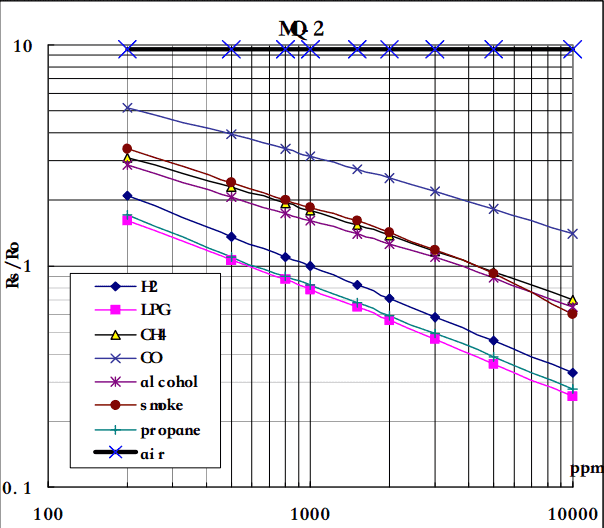
\includegraphics[width=8cm]{MQ2}
	\caption{Charakterystyka MQ-2}
\end{figure}
\begin{figure}[ht]
	\centering
	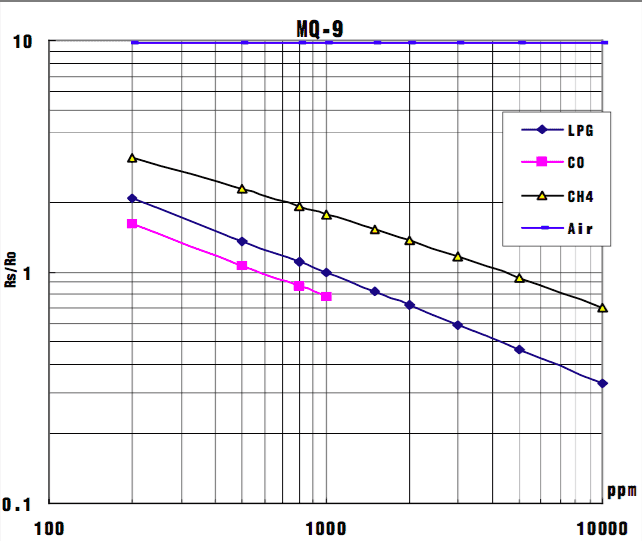
\includegraphics[width=8cm]{MQ9}
	\caption{Charakterystyka MQ-9}
\end{figure}
<<<<<<< HEAD
Niestety żaden model Raspberry nie posiada wbudowanego przetwornika analogowo cyfrowego dlatego konieczne było użycie układu zewnętrzenego. Wybrano przetwornik MCP3008 ze względu na jego nisko koszt i interfejs SPI, który jest wspierany przez Raspberry Pi.
MCP3008 to 10-bitowy przetwornik analogowy cyfrowy. Zasilany jest napięciem 5V, napięcie VRef = 5V.  Skoro jest to przetwornik 10-bitowy jest w stanie wykryć 1024 stany. Wykrywana przez niego minimalna różnica napięć na wejściu wynosi 
\begin{equation}
1 * 5V / 1024 = 4.88mV
\end{equation}
Posiada 8 kanałów jednak w projekcie wykorzystano tylko 2 – dla czujników MQ-9 i MQ-2.
=======

Ro - jest to stała wartość oporu czujnika przy 1000ppm H2 w czystym powietrzu.
Rs - jest to opór czujnika w różnych stężeniach gazu.
Skoro Ro jest stałe to przy wzroście Rs czułość będzie maleć. Dlatego też im mniejszy stosunek Rs do Ro tym lepiej. Widać, że oba czujniki reagują na wiele różnych gazów. MQ-2 nazwano czujnikiem LPG a MQ-9 czujnikiem CO ze względu na to, że w stosunku do tych gazów mają najwyższą czułość. 

Niestety żaden model Raspberry nie posiada wbudowanego przetwornika analogowo cyfrowego dlatego konieczne było użycie układu zewnętrznego. Wybrano przetwornik MCP3008 ze względu na jego nisko koszt i interfejs SPI, który jest wspierany przez Raspberry Pi.
MCP3008 to 10-bitowy przetwornik analogowy cyfrowy. Zasilany jest napięciem 5V.  Skoro jest to przetwornik 10-bitowy jest w stanie wykryć 1024 stany. Posiada 8 kanałów jednak w projekcie wykorzystano tylko 2 – dla MQ-9 i MQ-2.
>>>>>>> 2688ba13846a92baa8deea770d60be5065fe7915
\paragraph{Interfejs SPI:}
\begin{figure}[ht]
	\centering
	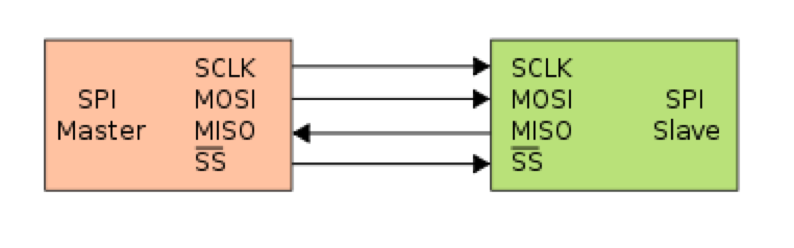
\includegraphics[width=5cm]{SPI.png}
	\caption{Interfejs SPI}
\end{figure}
SPI jest to interfejs synchroniczny (rys. 3.8). Może być do niego podłączone wiele urządzeń typu slave, jednak tylko z jednym urządzeniem Master, które generuje zegar. Master poprzez linię SS wybiera urządzenie z którym chce się komunikować.  \\
Interfejs ten zawiera jeszcze 3 linie:
\begin{enumerate} 
\item MOSI (ang. Master Output Slave Input): \\
Poprzez tę linię wysyłane są dane z Raspberry Pi do przetwornika analogowo cyfrowego MCP3008.
\item MISO (ang. Master Input Slave Output):\\
Poprzez tę linię wysyłane są dane z przetwornika AC do układu Master czyli w naszym przypadku Raspberry Pi 3
<<<<<<< HEAD
\item SCLK (ang. Serial CLocK) :\\
=======
\item SCLK (ang. Serial Clock) :\\
>>>>>>> 2688ba13846a92baa8deea770d60be5065fe7915
Ta linia wykorzystywana jest do przesłania zegara wygenerowanego przez Rapberry Pi 3
\end{enumerate}
Do komunikacji poprzez ten interfejs wykorzystano bibliotekę spiDev. \\
Każdy układ monitoruje wskaźniki pomiarowe z czujników analogowych i cyfrowych. W przypadku wykrycia wskazań, które w znaczący sposób odbiegają od normy informuje właściciela o zagrożeniu. Informacja ta wysyłana jest do wszystkich urządzeń(smartfony, tablety itp), które posiada właściciel.  Analizując dane z czujników analogowych w czystym powietrzu, które wynoszą wtedy odpowiednio:\\
Czujnik MQ-9: od 0.15 do 0.2\\
Czujnik MQ-2: od 0.05 do 0.15\\
Przyjęto, że granicą wysłania notyfikacji do użytkownika jest przekroczenie progu 0.3. Wartości te to znormalizowane dane z przetwornika AC, który jak już wcześniej wspomniano wykrywa 1024 stany. Odczytywane wartości bezpośrednio na wyjściu przetwornika MCP3008 dla czujnika MQ-9 w czystym powietrzu to około 170. Stąd 170/1024 = 0.166. Wysłanie notyfikacji wiąże się z otrzymaniem wartości większej niż 308.
<<<<<<< HEAD
Czujniki cyfrowe wykorzystane w pracy informują o wykryciu płomieni i ruchu. W przypadku detekcji takiego zagrożenia na wyjściu pojawia się stan niski i utrzymywany jest przez kilka sekund. W kodzie jednak wykonujemy instrukcje negacji, aby stan wysoki informował o niebezpieczeństwie a stan niski reprezentował jego brak. Na czujnikach znajduje się potencjometr, za pomocą którego dowolnie można ustawiać jego czułość. Odczyt danych następuje nieprzerwanie co 2 sekundy. Nie należy obawiać się, że czujnik ruchu nie wykryje zagrożenia z powodu braku odczytu we właściwym momencie, ponieważ utrzymuje on stan wysoki przez 5 sekund po wykryciu ruchu. Oprogramowanie wysyła także informacje z czujników do bazy danych Firebase. Zastosowanie takiej bazy daje możliwość monitorowania wszystkich danych w czasie rzeczywistym na aplikacjach klienckich. Dodatkowo w przypadku zagrożenia czyli przekroczeniu progu o którym mowa wyżej wysyłana jest push notyfikacja do urządzeń użytkownika a informacja o zagrożeniu zapisywana jest w bazie danych Django. Każdy jest w stanie odtworzyć całą historię wydarzeń w swoim systemie.
=======
Czujniki cyfrowe wykorzystane w pracy informują o wykryciu płomieni i ruchu. Czujnik ruchu detekcję zagrożenia określa przez stan wysoki natomiast czujnik płomieni przez stan niski. W kodzie jednak wykonano instrukcje negacji, aby stan wysoki informował o niebezpieczeństwie a stan niski reprezentował jego brak. Na czujnikach znajduje się potencjometr, za pomocą którego dowolnie można ustawiać jego czułość. Odczyt danych następuje nieprzerwanie co 2 sekundy. Nie należy obawiać się, że czujnik ruchu nie wykryje zagrożenia z powodu braku odczytu we właściwym momencie, ponieważ utrzymuje on stan wysoki przez 5 sekund po wykryciu ruchu. Oprogramowanie wysyła także informacje z czujników do bazy danych Firebase. Zastosowanie takiej bazy daje możliwość monitorowania wszystkich danych w czasie rzeczywistym na aplikacjach klienckich. Dodatkowo w przypadku zagrożenia czyli przekroczeniu progu, o którym mowa wyżej wysyłana jest push notyfikacja do urządzeń użytkownika a informacja o zagrożeniu zapisywana jest w bazie danych Django. Każdy jest w stanie odtworzyć całą historię wydarzeń w swoim systemie.
>>>>>>> 2688ba13846a92baa8deea770d60be5065fe7915
Aby zapewnić wydajny i pewny system bezpieczeństwa przy otrzymaniu wysokich wartości na czujnikach zapisywany jest czas zdarzenia. Każda kolejna notyfikacja zostanie wysłana po upływie 10 minut od poprzedniej przy założeniu, że stan na czujniku nadal jest wysoki. 

\section*{Obsługa wideo}

\paragraph{Protokół RTMP}
Podstawą funkcji strumieniowania wideo, jest protokół RTMP (Real-Time Message Protocol). Jest to, oparty na protokole TCP, protokół wysyłania obrazu, dźwięku oraz danych. 
Podstawową jednostką danych, w protokole RTMP, jest wiadomosć (ang. Message), której struktura jest zależna od typu strumieniowanych informacji. 
Wiadomosci dzielone są na kawałki (ang. Chunks), które są porcjami gotowymi do transmisji. Zatem strumień RTMP to ostatecznie strumień cząstek (ang. Chunk Stream)

Ponadto, wykorzystano protokół HLS (HTTP Live Streaming), zapisywanie odbieranego obrazu, we wskazanej liczbie plików wideo o okreslonej dłusgoci. Gdy aplikacja kliencka odtwarza strumień wideo, w rzeczywistosci odbiera, strumieniowane po kolei, zapisane pliki ts. Wpływa to na opóźnienie odtwarzania, względem rzeczywistosci, z jednej strony, a z drugiej, dostarcza płynne wideo.

\paragraph{h264}

<<<<<<< HEAD

=======
>>>>>>> 2688ba13846a92baa8deea770d60be5065fe7915
\paragraph{Raspberry Pi}
Do obsługi strumieniowania wideo, po stronie Raspberry Pi, wykorzystywany jest program FFMPEG. Pozwala on na sterowanie strumieniem, od wyboru urządzenia wejsciowego, przez statystyki strumienia, po punkt docelowy. Dostęp do unikatowego, dla każdego urządzenia Raspberry, punktu końcowego, gwarantowało wczeniejsze pobranie nr seryjnego urządzenia. Poniżej przedstawiono skrypt, wykonujący wymienione funkcje:
\begin{verbatim}
#!/bin/bash
serial_id="$(cat /proc/cpuinfo | grep Serial | cut -d ' ' -f 2)"
raspivid -o - -t 0 -fps 30 -b 1000000 | ffmpeg -re -ar 44100 -ac 2 -acodec pcm_s16le -f s16le -i /dev/zero -f h264 -i - -vcodec copy -g 60 -strict experimental -f flv rtmp://52.236.165.15:1936/camera/${serial_id}
\end{verbatim}
Pierwszą czynnoscią, wykonywaną w skrypcie, jest otwarcie pliku /proc/cpuinfo, następnie znajdowana jest w nim linia, w której znajduje się wyjątkowy serial urządzenia. Na końcu, z wykorzystaniem potoku, i funkcji cut, wartosć ta zostaje przypisana do zmiennej serial_id.

W drugiej linii skryptu wykorzystane jest narzędzie linii poleceń Raspberry - raspivid. Pozwala ono pobrać obraz z kamery. 
\begin{itemize}
\item Pierwszym przełącznikiem jest -o z parametrem -. Oznacza to, że obraz z kamery jest wysyłany na wyjscie standardowe.
\item Przełącznik -t ustawiony na 0 pozwala przekazywać obraz, z modułu kamery, przez nieokrelony czas. Aby przestać pobierać wideo, należy użyć przerwania za pomocą sygnału SIGINT (obsługiwanego w terminalu skrótem klawiszowym CTRL+C).
\item Opcja -fps pozwala wskazać liczbę przechwytywanych klatek w ciągu sekundy. Tutaj wykorzystano maksymalne możliwoci wybranego modułu kamery.
\item Ostatnią opcją, wykorzystaną w pobieraniu obrazu z kamery, jest bitrate, tzn wielkosć pamięci, w której ma się znaleźć obraz przechwycony w ciągu 1 sekundy. Ustawienie opcji -b na 1000000 oznacza, że 1 sekunda wideo, może zajmować 125 kilobajtów pamięci. Jest to szczególnie istotna informacja, w kontekcie transmisji obrazu poza urządzenie.
\end{itemize}

Drugim poleceniem jest wywołanie narzędzia ffmpeg, połączonego za pomocą potoku, odbierającego, przechwytywany za pomocą funkcji raspivid, obraz i przekazującego go na docelowy punkt końcowy. Za jego pomocą ustala się ostatecznie opcje kodujące obraz i dźwięk w trakcie końcowej transmisji.
\begin{itemize}
\item Przełącznik -re pozwala odczytywać dane wejsciowe, z oryginalną częstotliwoscią. Zatem zostają przechwycone ustawienia przełącznika funkcji raspivid -fps 30.
\item Opcje  -ar, -ac, -acodec, -f, -strict odpowiadają kolejno za: próbkowanie dźwięku, wybór liczby kanałów, kodek audio, format dźwięku oraz wybór eksperymentalnego sposobu kodowania. Wymuszenie wykorzystania, jako wejscia strumienia dźwięku, na /dev/zero, oznacza, że strumień ten zostaje wypełniony wartosciami pustymi. Zatem opcje transmisji dźwięku są nieistotne.
\item Przełącznik -vcodec ustala kodek wideo. W pracy wykorzystano standard kodowania h264.
\item Następnie ustawiono wejscie obrazu. Przełącznik -i - powoduje, że narzędzie ffmpeg przechwytuje, dzięki potokowi, obraz przekazywany funkcją raspivid.
\item Opcja -g 60 oznacza, że tzw klatka kluczowa (ang keyframe) pojawia się co 60 klatek. W tej sytuacji, co 2 sekundy. 
\item Przełącznik -f, w przypadku strumienia obrazu z kamery, wymusza format nadawanego wideo.  
\item Ostatnim elementem polecenia jest podanie punktu docelowego dla strumienia. Za pomocą protokołu RTMP, obługiwanego przez serwer o adresie IP 52.236.165.15 na porcie 1936, obraz wysyłany jest na aplikację o nazwie camera i punkt charakteryzowany przez serial urządzenia. Działanie tego elementu opisano w kolejnym punkcie. 
\end{itemize}

\paragraph{Serwer}
Narzędziem, umożliwiającym obsługę strumieniowanie wideo z wielu źródeł, na wiele urządzeń równoczesnie, jest serwer NGINX wraz z dodatkiem o nazwie rtmp-NGINX.

    \chapter{Rozwiązania chmurowe}

\section*{Microsoft Azure}

Aby zapewnić wysoki poziom bezpieczeństwa oraz dostępności systemu zdecydowano się na skorzystanie z chmury Micrsoft Azure.

\section*{Firebase}

// Mateusz

\section*{Aplikacja serwerowa}

// Ola

\section*{Baza danych}

// Ola
    \chapter{Aplikacje klienckie}

Na podstawie statystyk rynkowych, dostępnych na stronie statcounter.com (http://gs.statcounter.com/os-market-share/mobile-tablet/worldwide/#monthly-201801-201801-bar) zdecydowano się na stworzenie 3 klientów systemu The Guard, które umożliwią użytkowanie możliwie największej grupie osób:
\newline
\newline
\textbullet \space aplikacji mobilnej na system Android,\newline
\textbullet \space aplikacji mobilnej na system iOS,\newline
\textbullet \space aplikację webową.

\section*{Aplikacja Android}
\subsection*{Wybór narzędzi}
Do stworzenia aplikacji mobilnej na system Android użyto języka Kotlin - języka stworzonego przez firmę JetBrains, który 17.05.2017 r. (źródło: https://twitter.com/Android/status/864911929143197696) został uznany przez Google jako oficjalny język programowania aplikacji na platformę Android.
Kotlin ściśle współegzystuje z kodem stworzonym w Javie i w przypadku Androida jest kompilowany do kodu JVM.

Skorzystano ze środowiska Android Studio w wersji 3.0.1, do automatyzacji budowy projektu został wykrozystany Gradle w wersji 4.1.

Aplikacja skierowana jest na urządzenia z systemem Android od wersji Lollipop 5.0 (o numerze SDK większym niż 20), który został wydany 12.12.2014 r. Ograniczenie wersji spowodowane jest możliwością użycia bardziej zaawansowanych komponentów, niedostępnych dla niższych wersji. W styczniu 2018 r. oficjalne statystyki informują o tym, że około 80,7 \% wszystkich urządzeń z systemem Android na świecie ma wersję 5.0 lub wyższą.

\subsection*{Architektura}
Aplikacja The Guard dla systemu Android została stworzona zgodnie z założeniami architektury Model View Presenter. Architektura MVP zakłada rozdzielenie kodu źródłowego aplikacji na 3 kategorie:

\newline
\newline
\textbullet \space *Model*, czyli kod odpowiedzialny za logikę biznesową, połączenie z serwerem i złożone operacje,\newline
\textbullet \space *View*, czyli kod odpowiedzialny wyłącznie za poprawne wyświetlanie przygotowanych informacji,\newline
\textbullet \space *Presenter*, czyli kod odpowiedzialny za przygotowanie informacji otrzymanych z warstwy model do wyświetlenia w warstwie View.\newline

\newline Największą zaletą architektury MVP jest możliwość wygodnego testowania logiki aplikacji (w warstwie Presenter) oraz zastosowanie programowania reaktywnego przy użyciu biblioteki RxKotlin.

\subsection*{Interfejs użytkownika}
Tak zwane międzymordzie - kilka screenów i opis z linkiem do material design.

\subsection*{Integracje}
Opis połączenia aplikacji z Firebase, Fabric i innymi bibliotekami.

\begin{figure}[h]
    \centering
    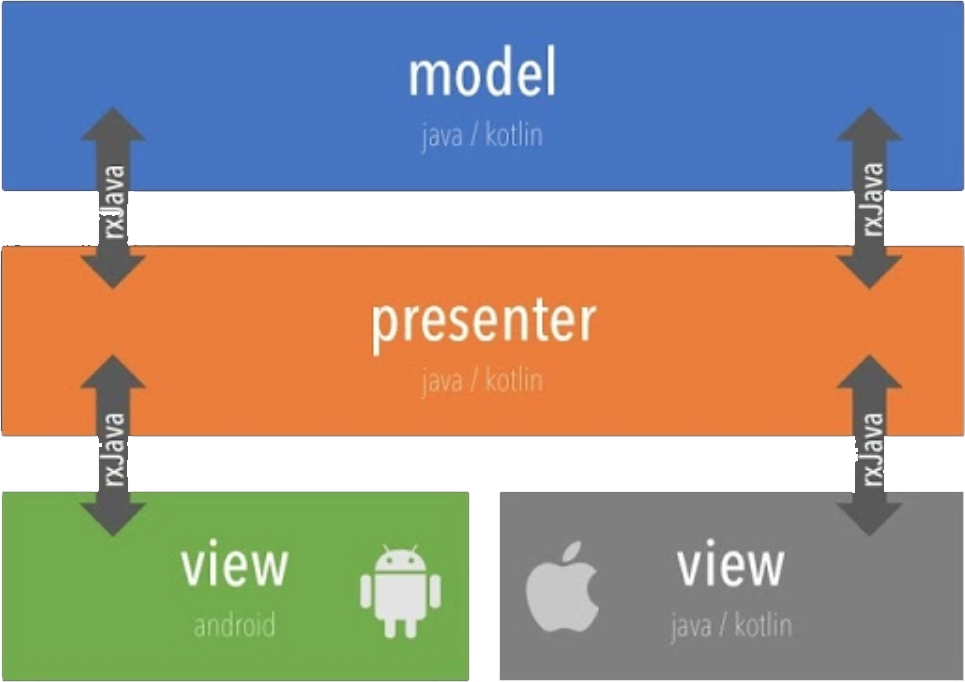
\includegraphics[width=9cm]{android_architecture}
    \caption{Architektura MVP}
\end{figure}

\section*{Aplikacja iOS}
Aplikacja przeznaczona jest na urządzenia z systemem operacyjnym iOS od wersji 10.0. 
Nie wspiera ona wcześniejszych wersji ze względu na nowe funkcje, które Apple wprowadziło wraz z pojawieniem się iOS 10.0 (m.in. klasa UNUserNotificationCenter). Jednak 92\% wszystkich obecnych użytkowników tego systemu(rys. 5.1) jest w stanie zainstalować aplikację a liczba ta stale rośnie. Aplikacja wspiera zarówno telefony komórkowe iPhone jak i tablety iPad. 
\begin{figure}[h]
	\centering
	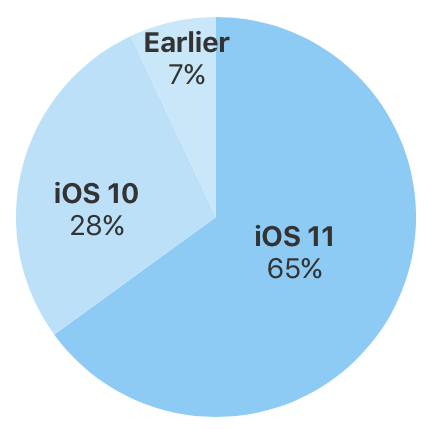
\includegraphics[width=6cm]{iOSstat}
	\caption{Udziały wersji systemu iOS w rynku}
\end{figure}
Napisana w stosunkowo nowym języku Swift (zaprezentowany przez Apple w 2014r na konferencji WWDC) w oparciu o architekturę MVC (Model-View-Controller) wykorzystując przy tym programowanie reaktywne i funkcjonalne. Aplikacja powstała w programie Xcode. Programowanie reaktywne zrealizowano przy pomocy biblioteki RxSwift. Ten paradygmat programowania związany jest z pojęciem obserwatora i sekwencji obserwowalnych. Każdy obserwator wywołując funkcję 'subscribe' na elemencie obserwowalnym otrzymuje informację o każdej zmianie na tym obiekcie. RxSwift wykorzystano m.in w celu wznowienia streamu obrazu z kamery w momencie przejścia aplikacji z trybu background do trybu foreground. Oznacza to, że po wyjściu z aplikacji, ale pozostawiając ja działającą w tle i po ponownym jej uruchomieniu tracono obraz ze streamu. Przyczyną jest polityka Apple, która nie zaleca aby aplikacje pracowały w tle i domyślnie wyłącza każdą taką aktywność. Ma to na celu przedłużenie żywotności baterii i optymalizacji całego systemu poprzez ograniczenie ilości zajmowanych zasobów [https://developer.apple.com/library/content/documentation/iPhone/Conceptual/iPhoneOSProgrammingGuide/BackgroundExecution/BackgroundExecution.html].  Oczywiście istnieje możliwość włączenia pracy w tle, jednakże konieczne jest aktywowanie trybu "Background Modes" i zaznaczenie konkretnej aktywności, którą chcielibyśmy wykonywać. Lista dozwolonych czynności możliwych do realizacji w tle jest ograniczona (rys. 5.2). 
\begin{figure}[h]
	\centering
	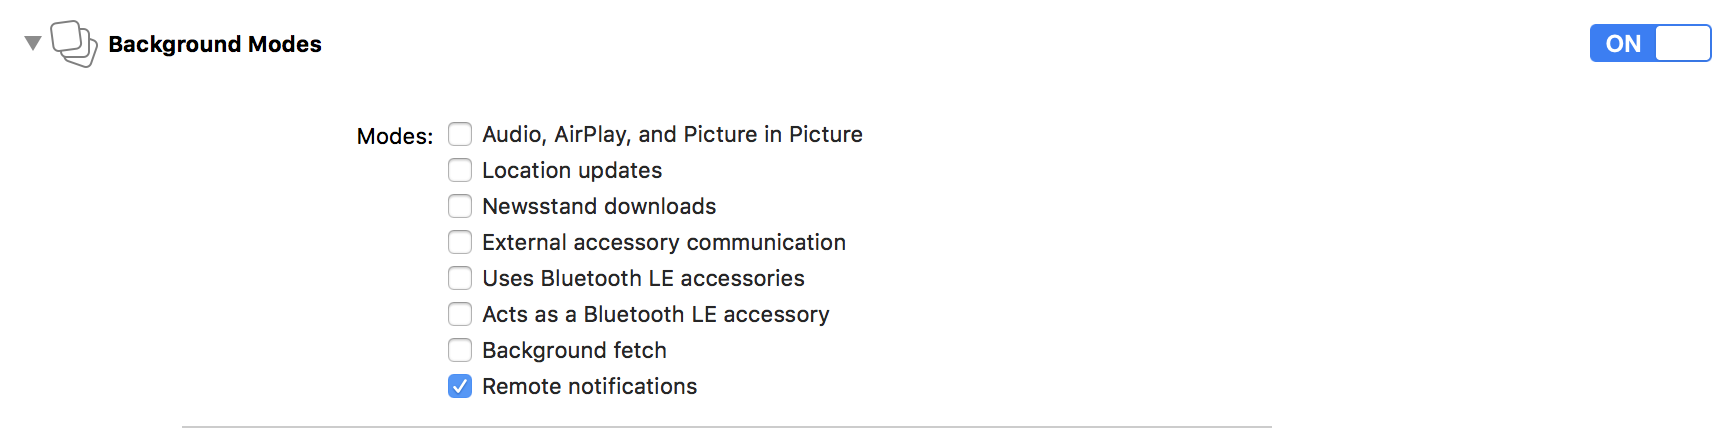
\includegraphics[width=9cm]{backgroundModes}
	\caption{Tryby pracy w tle}
\end{figure}
Próba oszustwa i wykonywania innej pracy w tle niż zaznaczona zostanie wychwycona w procesie weryfikacji przed jej publikacją na platformie Apple Store. Dzięki programowaniu reaktywnemu problem wznowienia podglądu obrazu został rozwiązany co prezentuje poniższy kod:
\begin{verbatim}
let appDelegate = UIApplication.shared.delegate as! AppDelegate
        appDelegate.inBackground.asObservable().subscribe(onNext: { (value) in
            if let streamView = self.streamView {
                if let player = self.currentPlayer {
                    if value == false {
                        self.streamVideoFrom(urlString: self.currentUrlString!)
                        print("Enter foreground")
                    } else {
                        print("Enter background")
                        streamView.layer.sublayers?.forEach({ (layer) in
                            layer.removeFromSuperlayer()
                        })
                    }
                }
            }
        }).disposed(by: disposeBag)
\end{verbatim}
Zmienna 'inBackground', która jest zmienną obserwowalną, ustawiana jest w oddzielnej klasie AppDelegate (klasa, która zapewnie poprawną interakcję z systemem iOS) na wartość true w chwili przejścia do trybu pracy w tle i na wartość false w przeciwnym wypadku. Klasa, w której wywoływany jest funkcja 'subscribe' jest obserwatorem tej zmiennej. Kod wewnątrz funkcji subscribe uruchamiany jest przy każdej zmianie wartości 'inBackground' i wznawia ponownie stream po każdym ponownym uruchomieniu programu.
"Programowanie funkcjonalne natomiast polega na traktowaniu funkcji jako obiektu. Oznacza to, że mogą być one zapisywane, kopiowane i przekazywane tak samo jak wszystkie inne obiekty. Mogą być używane jako parametry innych funkcji." [Pro Swift, Paul Hudson 04.19.2016 strona 172 link do store na iTunes : https://itunes.apple.com/us/book/pro-swift/id1111033310?mt=11 ]. Wykorzystane są w miejscach gdzie konieczne jest przekształcanie danych:
\begin{verbatim}
lastNotification = notifications.array.sorted(by: { (n1, n2) -> Bool in
	n1.date > n2.date 
}).filter({ (notif) -> Bool in return notif.type == "PIRSensor"}).first
\end{verbatim}
Na tablicy z notyfikacjami zastosowano szereg kolejnych funkcji: posortowano je malejąco według daty, przefiltrowano w taki sposób aby wybrać tylko te o typie 'PIRSensor' czyli te pochodzące z czujnika ruchu. Na sam koniec wybrano tylko jeden pierwszy element z wybranych i wynik wpisano do zmiennej lastNotification. Ważne jest, że każda kolejna wywoływana funkcja np. filter, odbiera wynik poprzedniej. 

Strukturę kodu (rys. 5.3) podzielono na kilka osobnych, logicznych części. Folder Firebase zawiera model bazy danych czujników, które zapisane są na serwerach Firebase. W folderze GuardManager znajdują się elementy odpowiedzialne za komunikację REST-ową z serwerem Django i modele bazy danych znajdującej się na naszym serwerze. Folder Views jest zbiorem widoków, które wczytywane są w zależności, w której sekcji się znajdujemy (opis sekcji niżej). ViewController.swift jest głównym kontrolerem zarządzającym widokami i modelami. Odpowiada za załadowanie odpowiedniego widoku i prezentację danych z odpowiedniej sekcji. W folderze GuardianAppTests napisane zostały testy jednostkowe, które sprawdzają poprawność przekształcania danych typu JSON (odpowiedź serwera) do obiektów zdefiniowanych w folderze GuardManager/Models. Klasy, których nazwy kończą się na Manager oznaczają obiekty typu Singleton. Celem takiego wzorca jest zapewnienie istnienia tylko jednej instancji w całej aplikacji i globalnego dostępu do tego obiektu. GuardManager, który odpowiada za pobieranie danych z bazy danych - taki obiekt nie powinien być utworzony więcej niż jeden raz, gdyż wszystkie klasy, które z niego korzystają nie potrzebują kolejnych instancji tej klasy. W ten sposób zapewniono, że zawsze odwołujemy się do tego samego obiektu.
\begin{figure}[h]
	\centering
	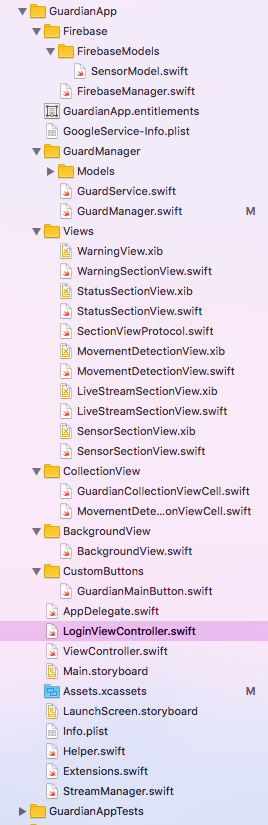
\includegraphics[width=4cm]{iOSstructure}
	\caption{Struktura aplikacji}
\end{figure}
Instalacja zewnętrznych bibliotek odbywa się za pomocą CocoaPods. Jest to menadżer zależności dzięki któremu szybko możemy wyszukać i zainstalować wymagane oprogramowanie. Wszystkie użyte zależności przedstawiono poniżej: 
\begin{verbatim}
  pod 'Moya'
  pod 'MBProgressHUD', '~> 1.0'
  pod 'RxSwift',    '~> 4.0'
  pod 'RxCocoa',    '~> 4.0'
  pod 'IHKeyboardAvoiding'
  pod 'Moya-SwiftyJSONMapper'
  pod 'Firebase/Core'
  pod 'Firebase/Messaging'
  pod 'Firebase/Auth'
  pod 'Firebase/Database'
  pod 'M13ProgressSuite'
\end{verbatim}
Moya używana jest do asynchronicznej REST-owej komunikacji z serwerem Django. SwiftyJSONMapper przydatna okazuje się do przekształcenia odpowiedzi serwera w postaci JSON do wcześniej zdefiniowanego modelu. MBProgressHUD umożliwia wyświetlanie ekranu ładowania podczas pobierania informacji z serwera. RxSwift i RxCocoa to biblioteki do programowania reaktywnego. Moduły Firebas/Core itp. służą do komunikacji z serwerami Firebase. Ostatni 'pod M13ProgressSuite' służy do rysowania wykresów i animowanych elementów graficznych w systemie iOS.
Po uruchomieniu aplikacji pierwszym widokiem jest ekran logowania i rejestracji użytkowników (rys 5.4). 
\begin{figure}[h]
	\centering
	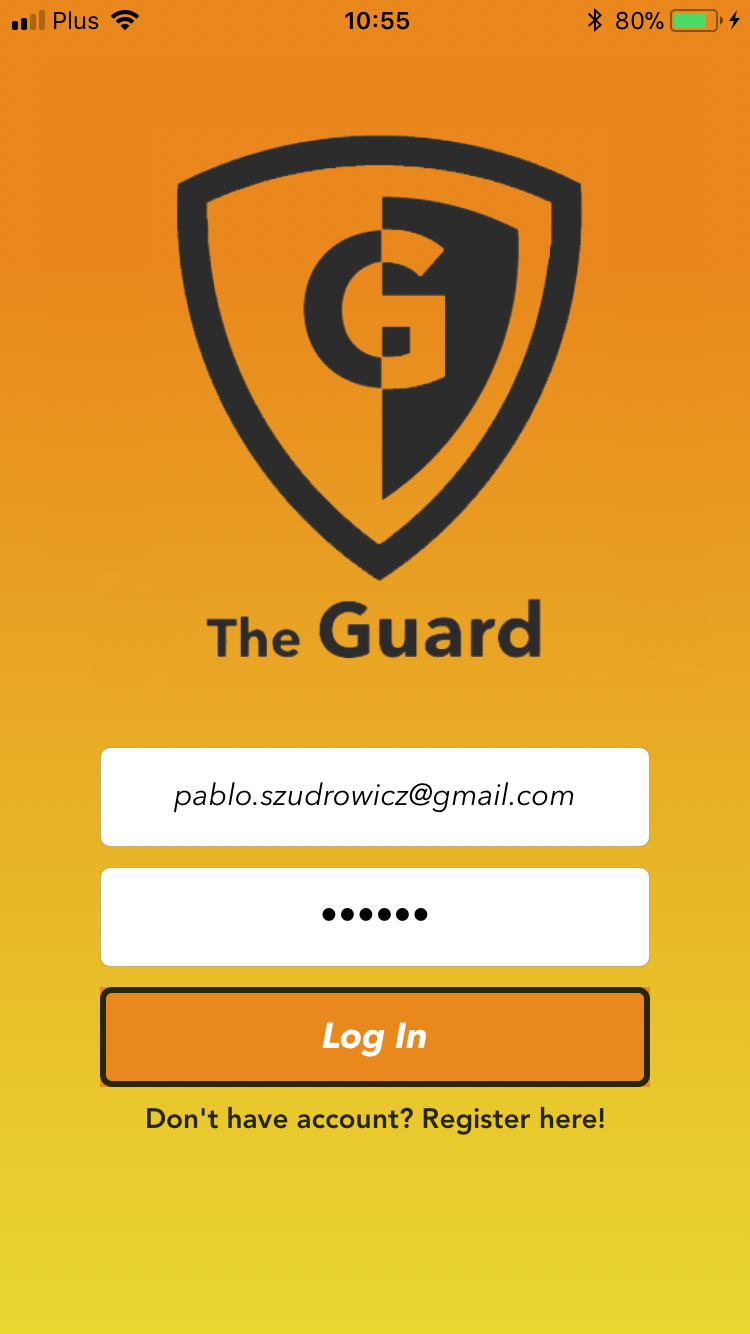
\includegraphics[width=5cm]{login.png}
	\caption{Ekran logowania}
\end{figure}
Po prawidłowym uwierzytelnieniu użytkownika uzyskiwany jest dostęp do głównego widoku aplikacji. W górnej części możliwy jest wybór 5 sekcji:
sekcja czujników, sekcja historii notyfikacji, sekcja ostatnich zagrożeń przy wykryciu ruchu, sekcja streamu na żywo, sekcja ustawień. Wszystkie te sekcje dotyczą konkretnego urządzenia wybranego w pasku na dole ekranu. Przy pierwszym uruchomieniu nie istnieje żadne urządzenie przypisane do naszego konta użytkownika. Aby dodać pierwsze i kolejne stacje, od których chcemy otrzymywać notyfikacje o zagrożeniach a także śledzić i monitorować informacje z czujników należy wybrać przycisk "New" z plusikiem w dolnej części ekranu. Pojawi się okno z prośbą o wpisanie numeru identyfikującego urządzenie. Po chwili dodany "Guard" będzie widoczny w na liście.
\paragraph{Sekcja czujników:}
Jest to jedna z najważniejszych sekcji aplikacji (rys 5.5).  Otrzymuje ona dane z czujników w czasie rzeczywistym i prezentuje je użytkownikowi.  W zależności od koloru prezentowanej wartości z czujnika użytkownik analizuje zagrożenie. Kolor zielony reprezentuje bezpieczne i prawidłowe odczyty na czujnikach, kolor pomarańczowy średnie, kolor czerwony reprezentuje bardzo wysoki poziom niebezpieczeństwa. Implementacja tej funkcjonalności zrealizowana została przy pomocy modelu HSV, który w przeciwieństwie do RGB pozwala na bardzo proste przejście z jednego koloru do kolejnego poprzez zmienę tylko jednego parametru. Zmieniając parametr Hue zmieniamy barwę przy stałym nasyceniu i jasności. Wartość tego parametru równa 120\textdegree{} odpowiada kolorowi zielonemu, kolor czerwony to 0\textdegree{}. Przekształcając wartość otrzymaną z czujników, która jest z zakresu [0-1] na wartość z przedziału [120-0] otrzymano wspomniany efekt. 
Poniżej przedstawiono fragment konwersji danych z czujników na kolor w modelu HSV, gdzie zmienna sensors[0] reprezentuje czujnik LPG.
\begin{verbatim}
UIColor(hue: CGFloat(0.33 - (sensors[0].value * 0.33)),
saturation: 1, brightness: 1, alpha: 1)
\end{verbatim}
\begin{figure}[h]
	\centering
	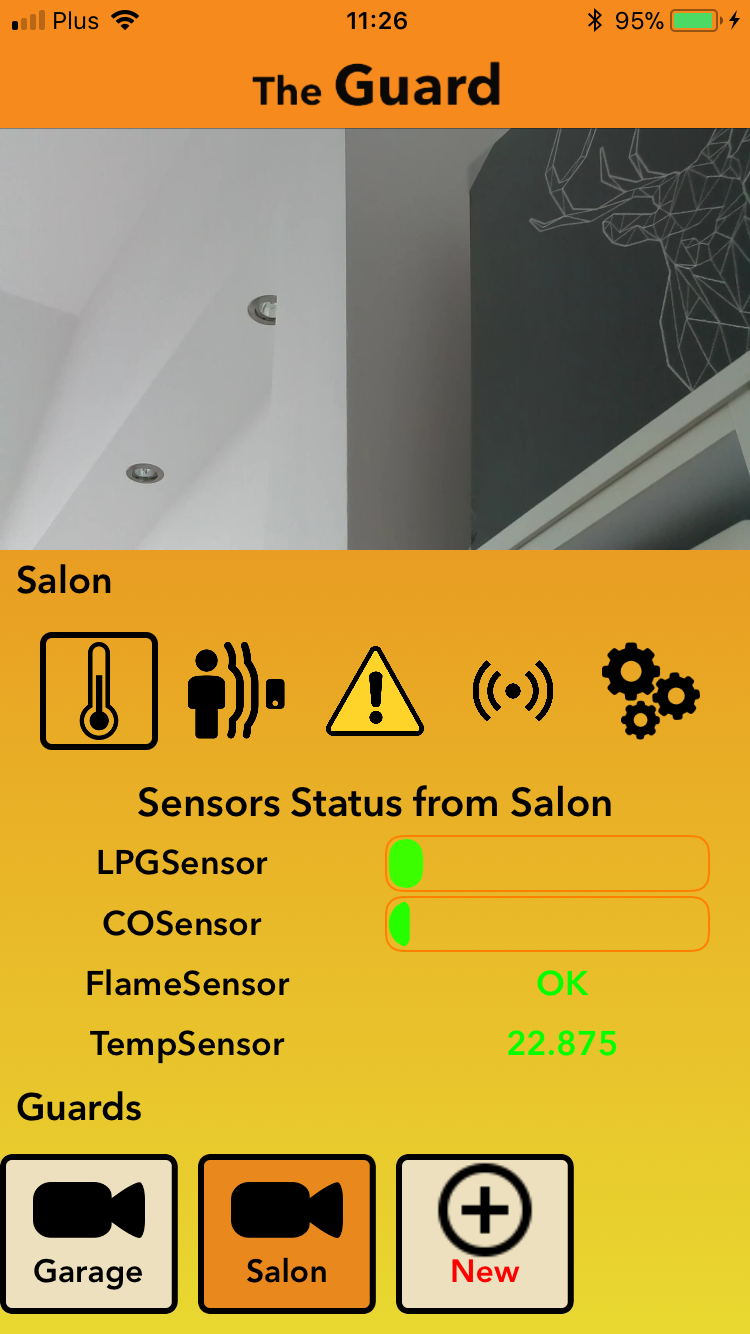
\includegraphics[width=5cm]{sensors.png}
	\caption{Sekcja czujników}
\end{figure}
\paragraph{Sekcja historii notyfikacji:}
W tej sekcji użytkownik ma dostęp do historii zdarzeń w systemie (rys 5.6). Po zaznaczeniu daty reprezentującej moment wystąpienia zagrożenia i wybranu przycisku 'preview' prezentowana jest informacja o miejscu niebezpieczeństwa i jego rodzaju. 
\begin{figure}[h]
\centering
\begin{minipage}{.4\linewidth}
    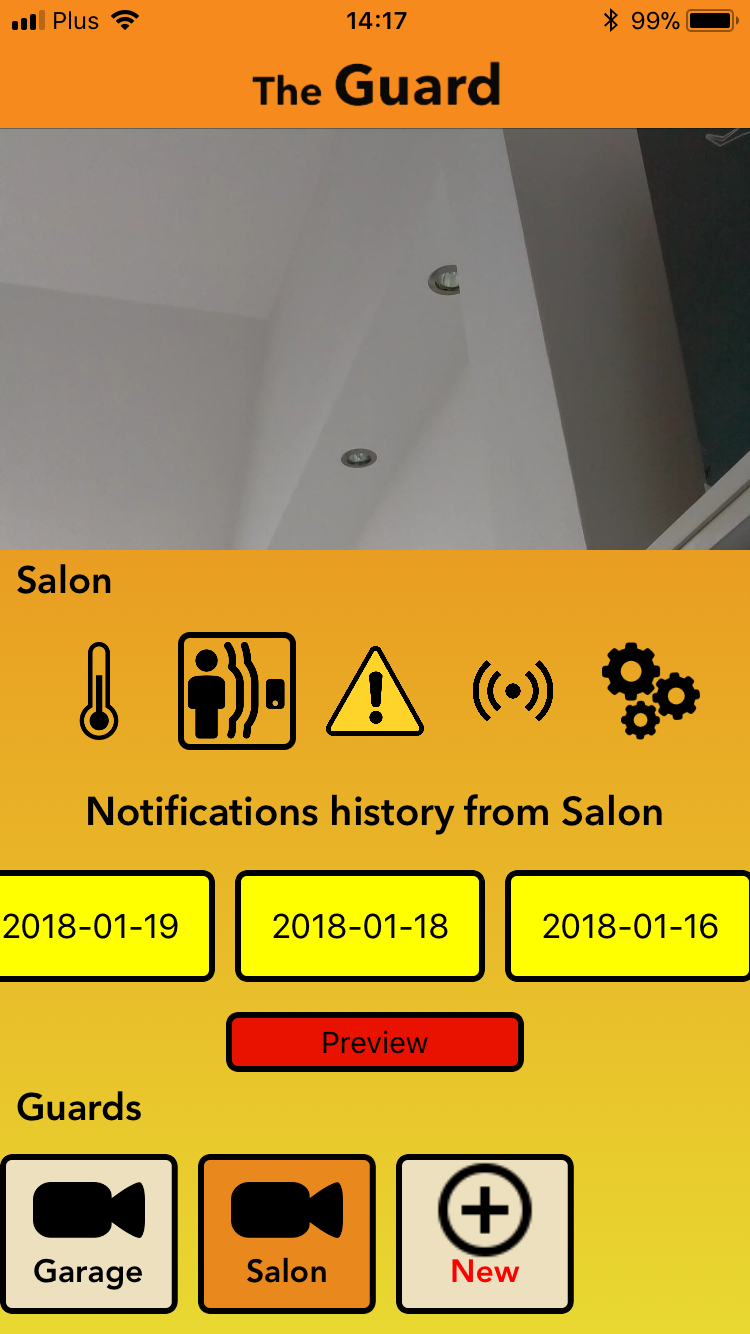
\includegraphics[width=\linewidth]{history.png}
    \caption{Sekcja historii notyfikacji}
    \label{img1}
\end{minipage}
\hspace{.05\linewidth}
\begin{minipage}{.4\linewidth}
    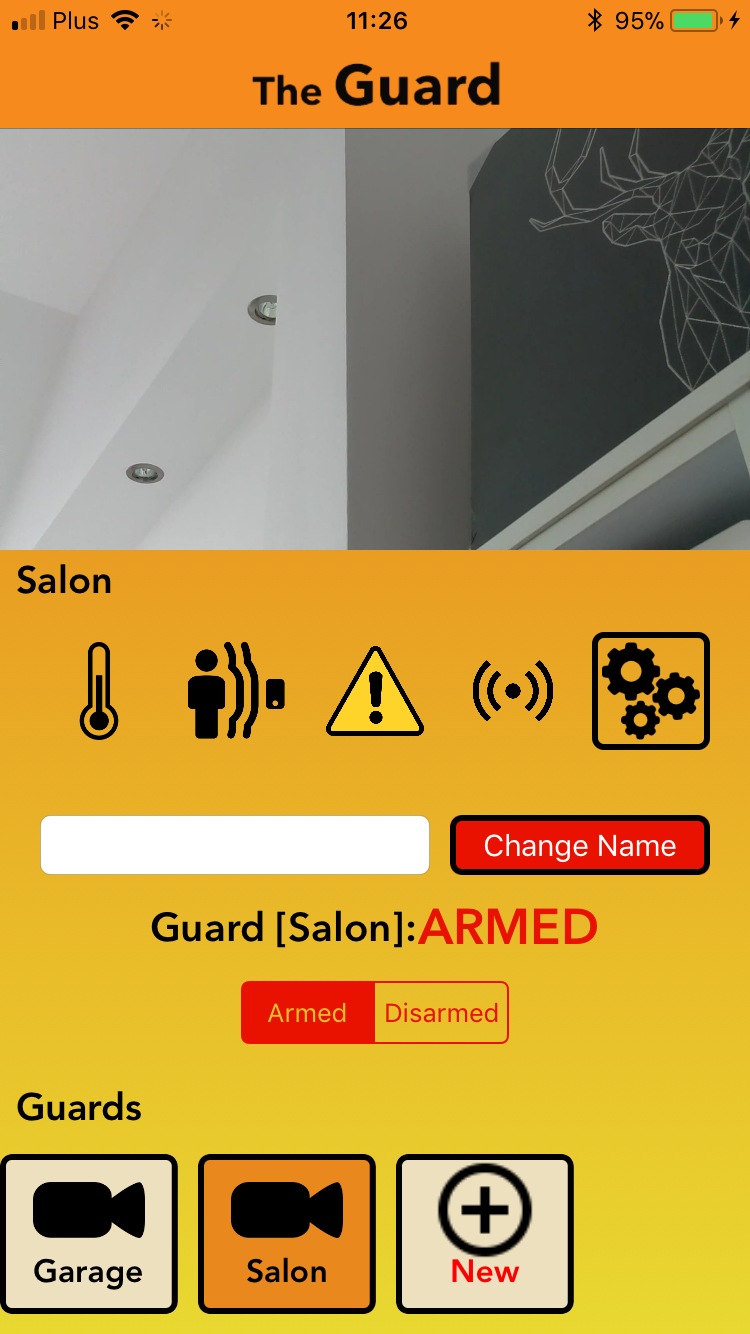
\includegraphics[width=\linewidth]{settings.png}
    \caption{Sekcja ustawień}
    \label{img2}
\end{minipage}
\end{figure} 
\paragraph{Sekcja ustawień:}
Użytkownik ma możliwość zmiany nazwy urządzenia, które zazwyczaj reprezentuje miejsce, w którym się znajduje. Istnieje również możliwość uzbrojenia i wyłączenia każdego urządzenia. Sprowadza się to do tego, że w przypadku zaznaczenia opcji "Disarmed" użytkownik nie otrzyma kolejnych notyfikacji o zagrożeniach (rys. 5.7). Opcja ta może okazać się przydatna w momencie uszkodzenia któregoś z modułów i tym samym błędnych danych wysyłanych z czujników.
\paragraph{Sekcja streamu:}
Sekcja odpowiedzialna za prawidłowy odbiór obrazu z kamery zaznaczonej w dolnej części ekranu. Okno, w którym odbywa się stream ustawiono w taki sposób, aby bez względu na rozmiar telefonu utrzymywało proporcję 16:9. Pozbyto się dzięki temu czarnych ramek lub braku części obrazu ze streamu.
\paragraph{Sekcja ostatnich zagrożeń:}
Sekcja prezentuje ostatnie nagrane zagrożenie. Służy do szybkiego przeglądu ostatniego niebezpieczeństwa i prezentuje ostatni nagrany materiał video. 

Przeprowadzono kilka testów aplikacji pod pełnym obciążeniem za pomocą programu Instruments. Szczególnie interesująco przedstawia się zużycie sieci podczas streamu obrazu. Widać, że w ciągu jednej minuty pobrano 6,61MB a wysłano jedynie 24,11Kb (rys. 5.8). Obraz pobierany jest tylko wtedy kiedy aplikacja jest aktywna. W ciągu godziny działania aplikacji pobierze ona około 400MB danych. Jednak dla zapewnienia komfortu użytkowania i płynnego streamu obrazu zalecane jest posiadanie łącza umożliwiającego transfer danych na poziomie min. 200KB/s. 
\begin{figure}[h]
	\centering
	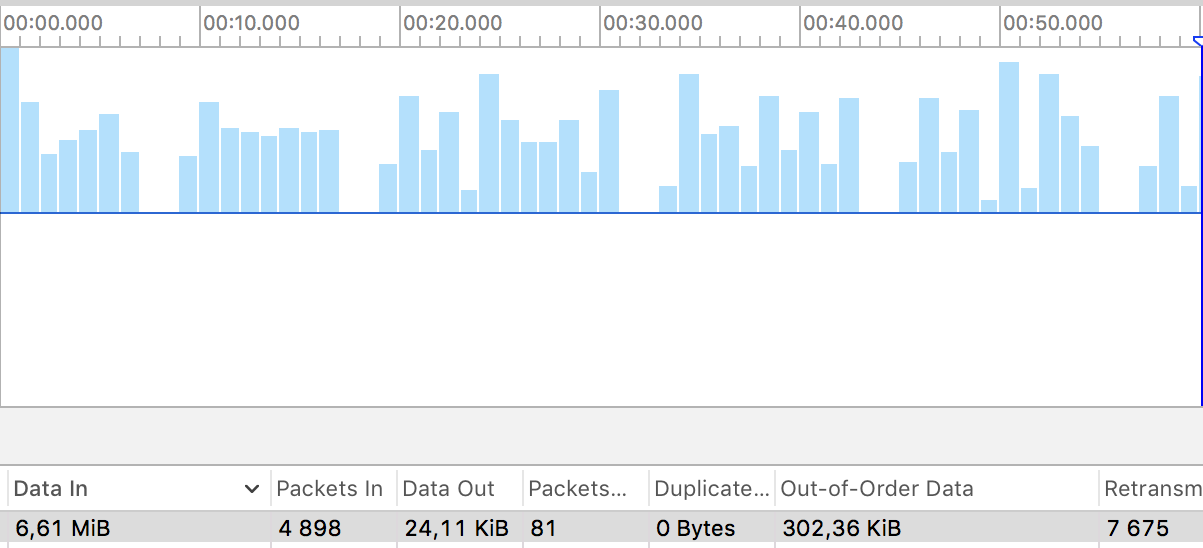
\includegraphics[width=11cm]{networkUsage}
	\caption{Zużycie sieci podczas streamu}
\end{figure}
Przeprowadzono także test na zużycie pamięci RAM i zużycie procesora. Te jednak są niewielkie i wynoszą odpowiednio 25MB pamięci RAM i średnio 1 procent zużycia procesora.
Zużycie procesora wzrasta do poziomu ok. 15 procent tylko w momencie pobierania nagranego obrazu z serwera. Wtedy też zużycie pamięci RAM jest o około 5MB większe i wynosi około 30MB (rys. 5.9).
\begin{figure}[h]
	\centering
	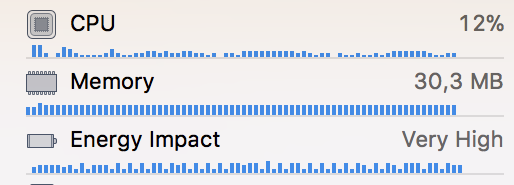
\includegraphics[width=11cm]{CPURAM}
	\caption{Zużycie procesora i RAM podczas największego obciążenia}
\end{figure}
Testy przeprowadzono na iPhonie 6S i iPadzie Pro.


\section*{Aplikacja internetowa}
Aplikacja webowa przeznaczona jest dla użytkowników wszystkich systemów operacyjnych i~została przetestowana w~przeglądarce Firefox. Rozmieszczenie komponentów aplikacji różni się od tego zastosowanego w~aplikacjach IOS oraz Android - spowodowane jest to inną rozdzielczością ekranu. 

\paragraph{Panel logowania / rejestracji użytkownika:}
\paragraph{Menu wyboru urządzenia:}
\paragraph{Główny panel aplikacji:}
\paragraph{Panel rejestracji urządzenia:}
\paragraph{Panel notyfikacji:}


\paragraph{Implementacja Django - połączenie z bazą danych:}
Biblioteka Django posiada wbudowane rozwiązania umożliwiające pobieranie informacji z bazy danych projektu dzięki czemu aplikacja webowa nie wysyła zapytań na określone dla aplikacji mobilnych porty, tylko komunikuje się bezpośrednio z bazą danych. Rozwiązanie to umożliwia uniezależnienie aplikacji webowej od stanu portów oraz zmniejsza liczbę potrzebnych zapytań wysyłanych do serwera.
    \chapter{Zakończenie}

Zakończenie pracy zwane również Uwagami końcowymi lub Podsumowaniem powinno zawierać ustosunkowanie
się autora do zadań wskazanych we wstępie do pracy, a w szczególności do celu i zakresu pracy oraz
porównanie ich z faktycznymi wynikami pracy. Podejście takie umożliwia jasne określenie stopnia
realizacji założonych celów oraz zwrócenie uwagi na wyniki osiągnięte przez autora w ramach jego
samodzielnej pracy.

Integralną częścią pracy są również dodatki, aneksy i załączniki np.~płyty CDROM
zawierające stworzone w ramach pracy programy, aplikacje i projekty.


    % All appendices and extra material, if you have any.
    \cleardoublepage\appendix%
    \chapter{Parę słów o stylu \texttt{ppfcmthesis}}

\section{Różnice w stosunku do ,,oficjalnych'' zasad składu ze stron FCMu}

Autor niniejszego stylu nie zgadza się z niektórymi zasadami wprowadzonymi w oficjalnym
dokumencie FCMu.\footnote{\url{http://www.fcm.put.poznan.pl/platon/dokumenty/dlaStudentow/egzaminDyplomowy/zasadyRedakcji}}
Poniższe elementy są składane nieco inaczej w stosunku do ,,oficjalnych'' wytycznych.

\begin{itemize}
    \item Promotor na stronie tytułowej jest umiejscowiony w centralnej osi pionowej strony (a
    nie po prawej stronie).

    \item Czcionka użyta do składu to nie Times New Roman.

    \item Spacje między tytułami akapitów oraz wcięcia zostały pozostawione takie, jak są zdefiniowane
    oryginalnie w pakiecie Memoir (oraz w \LaTeX{}u). Jeśli zdefiniowano ,,polską'' opcję składu,
    to będzie w użyciu wcięcie pierwszego akapitu po tytułach rozdziałów. Przy składzie ,,angielskim''
    tego wcięcia nie ma.

    \item Odwrócona jest kolejność rozdziałów \emph{Literatura} i \emph{Dodatki}.

    \item Na ostatniej stronie umieszczono stopkę informującą o prawach autorskich i programie
    użytym do składu.

    \item Nie do końca zgadzam się ze stwierdzeniem, iż ,,zamieszczanie list tabel, rysunków,
    wykresów w pracy dyplomowej jest nieuzasadnione''. Niektóre typy publikacji zawierają tabele i rysunki, których
    skorowidz umożliwia łatwiejsze ich odszukanie. Ale niech będzie.

    \item Styl podpisów tabel jest taki sam, jak rysunków i odmienny od FCMowego.
    Jeśli ktoś koniecznie chce mieć zgodne z wytycznymi
    podpisy, to zamiast \texttt{caption} niech użyje \texttt{fcmtcaption} do podpisywania tablic oraz
    \texttt{fcmfcaption} do podpisywania rysunków. Podpisy pod rysunkami pozostaną pełne, a nie skrócone (,,Rys.'').

    \item Styl formatowania literatury jest nieco inny niż proponowany przez FCM.
\end{itemize}



\end{document}

    \chapter{Składanie dokumentu w systemie \LaTeX}

Po pierwsze to gratulacje --- dobry wybór. W tym rozdziale znajduje się
garść informacji o tym, jak poprawnie składać tekst pracy w systemie \LaTeX{} wraz z
przykładami, które mają służyć do przeklejania do własnych dokumentów.

\section{Narzędzia}
Pracując pod systemem Windows, polecam:
\begin{itemize}
    \item MikTeX, \url{http://www.miktex.org/},
    \item JEdit, \url{http://www.jedit.org/},
    \item Ghostview, Ghostscript (podgląd dokumentów PDF bez blokowania pliku):\\
    \url{http://www.cs.wisc.edu/~ghost/}.
\end{itemize}

Po zainstalowaniu tych narzędzi wystarczy wykonać polecenie \texttt{compile.bat} (który
jest skryptem wsadowym dla Windows). Dla tych, którzy wolą nieco automatyzacji --- skrypt
\texttt{latexmk}, który jest w MikTeXu (a który potrzebuje zainstalowanego Perla) jest
również bardzo wygodny: \texttt{latexmk -pdf -pvc main.tex}.

\section{Edycja tekstu}
\chaptermark{Tytuł rozdziału, jeśli pełen się nie mieści\ldots{}}{}

\subsection{Struktura dokumentu}

Praca składa się z rozdziałów (\texttt{chapter}) i podrozdziałów (\texttt{section}).
Ewentualnie można również rozdziały zagnieżdzać (\texttt{subsection}, \texttt{subsubsection}),
jednak nie powinno się wykraczać poza drugi poziom hierarchii (czyli \texttt{subsubsection}).

\subsection{Akapity i znaki specjalne}

Każdy akapit to po prostu blok tekstu. Nieważne jak sformatowany --- to zrobi już
system $\LaTeX$.

Akapity rozdziela się od siebie przynajmniej jedną pustą linią. Podstawowe
instrukcje, które się przydają to \emph{wyróżnienie pewnych słów}. Można również
stosować \textbf{styl pogrubiony}, choć nie jest to generalnie zalecane.

Należy pamiętać o zasadach polskiej interpunkcji i ortografii. Po spójnikach
jednoliterowych warto wstawić znak tyldy ($\sim$), który jest tak zwaną
,,twardą spacją'' i powoduje, że wyrazy nią połączone nie będą rozdzielane
na dwie linie tekstu.

Polskie znaki interpunkcyjne różnią się nieco od angielskich: to jest ,,polski'', a to jest
``angielski''. W kodzie źródłowym tego tekstu będzie widać różnicę.

Proszę również zwrócić uwagę na znak myślnika, który może być pauzą ,,---'' lub
półpauzą: ,,--''. Należy stosować je konsekwentnie. Do łączenia wyrazów używamy
zwykłego ,,-'' (\emph{północno-wschodni}), do myślników --- pauzy lub półpauzy.
Inne zasady interpunkcji i typografii można znaleźć w słownikach.

\subsection{Wypunktowania}

Wypunktowanie z cyframi:
\begin{enumerate}
    \item to jest punkt,
    \item i to jest punkt,
    \item a to jest ostatni punkt.
\end{enumerate}

\noindent
Po wypunktowaniach czasem nie warto wstawiać wcięcia akapitowego. Wtedy przydatne jest
polecenie \texttt{noindent}. Wypunktowanie z kropkami (tzw.~\emph{bullet list}) wygląda tak:
\begin{itemize}
    \item to jest punkt,
    \item i to jest punkt,
    \item a to jest ostatni punkt.
\end{itemize}

\noindent
Wypunktowania opisowe właściwie niewiele się różnią:
\begin{description}
    \item[elementA] to jest opis,
    \item[elementB] i to jest opis,
    \item[elementC] a to jest ostatni opis.
\end{description}


\subsection{Polecenia pakietu \texttt{ppfcmthesis}}

Parę poleceń zostało zdefiniowanych aby uspójnić styl pracy. Są one przedstawione poniżej
(oczywiście nie trzeba się do nich stosować).

\paragraph{Makra zdefiniowane dla języka angielskiego.} Są nimi: \texttt{termdef} oraz \texttt{acronym}.
Przykłady poniżej obrazują ich przewidywane użycie w tekście.
\begin{center}
    \footnotesize%
    \begin{tabular}{l >{\rightskip\fill}p{12cm}}
        \toprule
        źródło & \texttt{we call this a $\backslash$termdef\{Database Management System\} ($\backslash$acronym\{DBMS\})} \\ \cmidrule(lr){2-2}
        docelowo & we call this a \termdef{Database Management System} (\acronym{DBMS}) \\
        \bottomrule
    \end{tabular}
\end{center}

\paragraph{Makra zdefiniowane dla języka polskiego.} Podobnie jak dla języka angielskiego zdefiniowano
odpowiedniki polskie: \texttt{defini\-cja}, \texttt{akronim} oraz \texttt{english} dla tłumaczeń angielskich
terminów. Przykłady poniżej obrazują ich przewidywane użycie w tekście.
\begin{center}
    \footnotesize%
    \begin{tabular}{l >{\rightskip\fill}p{12cm}}
        \toprule
        źródło & \texttt{nazywamy go $\backslash$definicja\{systemem zarządzania bazą danych\} ($\backslash$akronim\{DBMS\}, $\backslash$english\{Database Management System\})} \\ \cmidrule(lr){2-2}
        docelowo & nazywamy go \definicja{systemem zarządzania bazą danych} (\akronim{DBMS}, \english{Database Management System}) \\ \bottomrule
    \end{tabular}
\end{center}


\subsection{Rysunki}

Format wstawianych rysunków zależy od tego czy używa się do kompilacji polecenia
\texttt{latex}, czy też \texttt{pdflatex}. Oba powinny dać dokładnie ten sam wynik końcowy,
ale praca z nimi jest nieco inna.

\begin{description}
    \item[latex] To polecenie kompiluje źródła \LaTeX{}owe do pliku
    z rozszerzeniem \texttt{dvi}. Ten plik można przeglądać przy pomocy specjalizowanych programów
    takich jak przykładowo Yap obecny z dystrybucją Mik\TeX{}a. Aby uzyskać docelowy plik \akronim{PDF}
    należy przekonwertować plik \texttt{dvi} przy pomocy programu \texttt{dvipdfm}.

    \textbf{UWAGA:} korzystając z programu \texttt{latex}, wszystkie rysunki muszą być w formacie \akronim{EPS}
    (\english{encapsulated postscript}).

    \item[pdflatex] To polecenie kompiluje źródła \LaTeX{}owe bezpośrednio do pliku \akronim{PDF}.

    \textbf{UWAGA:} korzystając z programu \texttt{pdflatex}, wszystkie rysunki muszą być w formacie \akronim{PDF},
    \akronim{JPG} lub \akronim{PNG}.
\end{description}

Można oczywiście używać obu systemów --- wtedy pliki rysunków muszą po prostu być dostępne w obu formatach.

Wszystkie rysunki (w tym również diagramy, szkice i inne) osadzamy w środowisku
\texttt{figure} i umieszczamy podpis \emph{pod} rysunkiem, w formie elementu \texttt{caption}. Rysunki powinny
zostać umieszczone u góry strony (osadzone bezpośrednio w treści strony zwykle utrudniają czytanie tekstu).
Rysunek~\ref{rys:plama} zawiera przykład pełnego osadzenia rysunku na stronie.

\begin{figure}[t] % możliwe opcje to 't' - top, 'b' - bottom, 'h' - 'here', ale zaleca się 't'
    \centering
\includegraphics[width=5cm]{figures/template/logo-pp}
    \caption{Logo Politechniki Poznańskiej.}\label{rys:plama}
\end{figure}

\begin{figure}[t]
    \centering
\includegraphics[width=5cm]{figures/template/logo-pp}
    \fcmfcaption{Logo Politechniki Poznańskiej. Formatowanie zgodne z wytycznymi FCMu.}\label{rys:plama2}
\end{figure}

Zasady FCMu sugerują nieco inne nagłówki rysunków. Dostepne są one poleceniem \texttt{fcmfcaption} (zob.~rysunek
\ref{rys:plama2}), jeśli ktoś woli mieć podpisy niespójne z rysunkami\ldots

\subsection{Tablice}

Tablice to piękna rzecz, choć akurat ich umiejętne tworzenie w \LaTeX{}u nie jest łatwe.
Jeśli tablica jest skomplikowana, to pewnie łatwiej będzie ją wykonać w programie
OpenOffice, a następnie wyeksportować jako plik \akronim{PDF}. W każdym przypadku tablice wstawia się podobnie
jak rysunki, tylko że w środowisko \texttt{table}. Tradycja typograficzna sugeruje umieszczenie opisu tablicy, a więc
elementu \texttt{caption} ponad jej treścią (inaczej niż przy rysunkach).

Tablica~\ref{tab:tabela} pokazuje pełen przykład.

\begin{table}[h]
    \caption{Przykładowa tabela. Styl opisu jest zgodny z rysunkami.}\label{tab:tabela}
    \centering\footnotesize%
    \begin{tabular}{l c}
        \toprule
        artykuł & cena [zł] \\
        \midrule
        bułka & $0,4$ \\
        masło & $2,5$ \\
        \bottomrule
    \end{tabular}
\end{table}

Zasady FCMu sugerują nieco inne nagłówki tablic. Dostepne są one poleceniem \texttt{fcmtcaption} (zob.~tablicę
\ref{tab:tabela2}), jeśli ktoś woli mieć podpisy niespójne z rysunkami\ldots

\begin{table}[h]
    \fcmtcaption{Przykładowa tabela. Styl opisu jest zgodny z wytycznymi FCMu.}\label{tab:tabela2}
    \centering\footnotesize%
    \begin{tabular}{l c}
        \toprule
        artykuł & cena [zł] \\
        \midrule
        bułka & $0,4$ \\
        masło & $2,5$ \\
        \bottomrule
    \end{tabular}
\end{table}


\section{Literatura i materiały dodatkowe}

Materiałów jest mnóstwo. Oto parę z nich:
\begin{itemize}
    \item \emph{The Not So Short Introduction\ldots}, która posiada również tłumaczenie
    w języku polskim.\\
    \url{http://www.ctan.org/tex-archive/info/lshort/english/lshort.pdf}

    \item Klasy stylu \texttt{memoir} posiadają bardzo wiele informacji o składzie tekstów
    anglosaskich oraz sposoby dostosowania \LaTeX{}a do własnych potrzeb.\\
    \url{http://www.ctan.org/tex-archive/macros/latex/contrib/memoir/memman.pdf}

    \item Nasza grupa dyskusyjna i repozytorium SVN są również dobrym miejscem aby zapytać
    (lub sprawdzić czy pytanie nie zostało już zadane).\\
    \url{https://ophelia.cs.put.poznan.pl/svn/put-latex/trunk}

    \item Dla łaknących więcej wiedzy o systemie \LaTeX{} podstawowym źródłem informacji
    jest książka Lamporta~\cite{Lamport:LDP85}. Prawdziwy \emph{hardcore} to oczywiście
    \emph{The \TeX{}book} profesora Knutha~\cite{Knuth:ct-a}.
\end{itemize}



    % Bibliography (books, articles) starts here.
    \bibliographystyle{plalpha}{\raggedright\sloppy\small\bibliography{bibliography}}

    % Colophon is a place where you should let others know about copyrights etc.
    \ppcolophon

\end{document}
